\RequirePackage{amsthm}
\documentclass[pdflatex,sn-basic]{sn-jnl}

\usepackage{lmodern}
\usepackage{amssymb}
\usepackage{mathtools}
\usepackage{array}
\usepackage{xcolor}
\usepackage{manyfoot}
\usepackage{booktabs}
\usepackage{enumitem}
\geometry{reset,left=2cm,right=2cm,top=2cm,bottom=2cm,bindingoffset=0cm}


\graphicspath{{paper/figures/}{figures/}}

\theoremstyle{thmstyleone}
\newtheorem{theorem}{Theorem}
\newtheorem{proposition}[theorem]{Proposition}
\newtheorem{corollary}[theorem]{Corollary}
\newtheorem{lemma}[theorem]{Lemma}

\theoremstyle{thmstyletwo}
\newtheorem{example}{Example}
\newtheorem{remark}{Remark}

\theoremstyle{thmstylethree}
\newtheorem{definition}{Definition}

\newcommand{\E}{\mathbb E}
\newcommand{\Pbb}{\mathbb P}
\newcommand{\R}{\mathbb R}
\newcommand{\N}{\mathbb N}
\newcommand{\1}{\mathbf 1}
\newcommand{\calF}{\mathcal F}
\newcommand{\calH}{\mathcal H}
\newcommand{\calG}{\mathcal G}
\newcommand{\calY}{\mathcal Y}
\newcommand{\KL}{\operatorname{KL}}
\newcommand{\supp}{\operatorname{supp}}
\newcommand{\argmax}{\operatorname*{arg\,max}}
\newcommand{\dd}{\,\mathrm d}

\begin{document}

\title[Predictive e-diagnostics for movement HMMs]{Predictive e-diagnostics for multi-state movement models: A theoretical framework for hidden Markov models}

\author[1]{\fnm{Aurélien} \sur{Nicosia}}
\affil[1]{\orgname{Université Laval}, \orgaddress{\country{Canada}}}

\abstract{Hidden Markov models are widely used to describe animal movement as a sequence of unobserved behavioural states generating observed step lengths, turning angles and other movement variables. Standard assessment workflows combine likelihood-based criteria, decoded state paths, simulation checks and graphical diagnostics. These tools are useful, but they do not by themselves give a sequentially valid account of adaptive model checking, nor do they distinguish clearly between observable predictive distributions and model-dependent reconstructions of latent states. This paper develops a theoretical framework for \emph{predictive e-diagnostics} in multi-state movement models. A fitted HMM is treated as a sequential generator of held-out movement data. Diagnostic alternatives are encoded as predictable one-step or blockwise predictive densities, and the corresponding density ratios define e-value increments. The latent state process is integrated out by filtering, so the denominator is the observable predictive density, not a density conditional on a decoded path. Under a fixed train/validation protocol, the cumulative product of predictive density ratios is a nonnegative supermartingale under the fitted null generator and hence an e-process. The paper extends this basic guarantee to optional stopping, predictable switching among diagnostic alternatives, weighted and state-localized e-processes, feature-level diagnostics based on residual or circular-linear transformations, blockwise long-horizon diagnostics and conservative composite-null envelopes. These results provide a principled basis for movement-specific diagnostics targeting the number of states, angular misspecification, residual step-angle dependence, duration structure, temporal nonstationarity and long-term generative behaviour.}

\keywords{Animal movement, hidden Markov model, e-value, e-process, sequential prediction, model diagnostics, filtering, circular data, anytime-valid inference}

\maketitle

\section{Introduction}

Hidden Markov models (HMMs) are a central tool for analysing animal movement data when movement is represented as the observable output of an unobserved behavioural state process. In many applications, observations are constructed from locations as step lengths and turning angles, and latent states are interpreted as behavioural modes such as resting, encamped movement, foraging, exploratory movement or directed travel. Early movement models based on mixtures of random walks formalized this idea using step lengths and turning angles \citep{morales_2004_relocation}. HMM-type extensions are now standard for animal telemetry and movement ecology \citep{langrock_2012_telemetry,zucchini_2016_hmm}, and software such as \texttt{moveHMM} \citep{michelot_2016_movehmm} and \texttt{momentuHMM} \citep{mcclintock_2018_momentuhmm} has made these models accessible in applied ecological work.

Model assessment for movement HMMs often relies on AIC or BIC, likelihood comparisons, inspection of decoded state paths, residual checks, simulation-based checks and ecological interpretation of inferred behaviours. These practices are useful, but they raise at least three statistical issues. First, diagnostics are often chosen after seeing the data, which makes the inferential status of repeated exploratory checking unclear. Second, the latent states are sometimes treated as if they were observed after decoding, even though decoded states remain model-dependent reconstructions. Third, a high fitted likelihood or a plausible state interpretation does not ensure that the model is a good sequential generator of future movement patterns, especially for long trajectories, held-out individuals, directional persistence, state dwell times or spatially aggregated summaries.

This paper proposes a predictive alternative. The fitted HMM is evaluated as a sequential generator of a validation trajectory. At each time $t$, the null model provides an observable predictive density
\[
 p_0(y_t \mid \calF_{t-1}).
\]
A diagnostic alternative provides another predictive density
\[
 q_t(y_t \mid \calF_{t-1}),
\]
chosen before $Y_t$ is observed. The ratio
\[
 E_t=\frac{q_t(Y_t\mid \calF_{t-1})}{p_0(Y_t\mid \calF_{t-1})}
\]
is a predictive e-value increment. Its cumulative product is an e-process under the null generator. The resulting evidence process can be monitored over time and compared with thresholds of the form $1/\alpha$, with the usual anytime-valid interpretation supplied by Ville's inequality \citep{ville_1939_collectif,howard_2020_time_uniform}. The construction connects movement-model diagnostics to the prequential view of statistical evaluation \citep{dawid_1984_prequential} and to the modern literature on e-values, safe testing and anytime-valid inference \citep{vovk_wang_2021_evalues,grunwald_2024_safe_testing}.

The main point is not simply to replace likelihood ratios by a new terminology. The contribution is to treat movement-model validation as a predictable sequence of diagnostic predictive alternatives (informally, ``bets'') against a fitted generator. This leads to several methodological consequences. The denominator must be the observable predictive density, obtained by filtering over latent states. Diagnostic alternatives may be switched or mixed predictably. Local evidence can be accumulated only over selected periods, habitats or soft state weights while preserving e-process validity. Movement-specific summaries, including circular residuals, step-angle dependence measures and blockwise spatial summaries, can be converted into feature-level e-values whenever their null predictive law is available or can be estimated on independent data.

The paper is written as a theoretical setup for a first methodological article. The core guarantees are exact under a fixed train/validation protocol. This means that the null model and diagnostic alternatives are fitted or specified before validation, and the validation sequence is then used only to compute predictive ratios. The same-sample workflow in which the analyst fits the model, chooses diagnostics and evaluates them all on the same observations is not covered by the exact guarantees below unless additional sample splitting, cross-fitting or pre-specified conditioning arguments are used.

The numerical section is deliberately focused. The main article reports the scenarios that support the core methodological message: calibration under a fixed null generator, targeted movement diagnostics, predictable localization and predictable diagnostic combination. Additional sensitivity checks and extensions are reported in the supplementary material.

\paragraph{Main contributions.}
The paper develops the following theoretical components.
\begin{enumerate}[label=(C\arabic*)]
\item A predictive e-process theorem for fixed movement HMMs evaluated on held-out validation sequences.
\item A filtering result showing that validity is based on marginal observable prediction, not on densities conditional on decoded state paths.
\item Optional-stopping, predictable-switching, mixture and sequential exploratory workflow results for diagnostic alternatives.
\item Weighted and state-localized e-processes that permit valid localization of model failure by time, habitat or predicted behavioural state.
\item Feature-level and blockwise e-diagnostics for circular-linear movement summaries and long-horizon generative checks.
\item A clear separation between exact split-sample validity, exploratory same-sample diagnostics and conservative composite-null extensions.
\end{enumerate}

\begin{figure}[t]
\centering
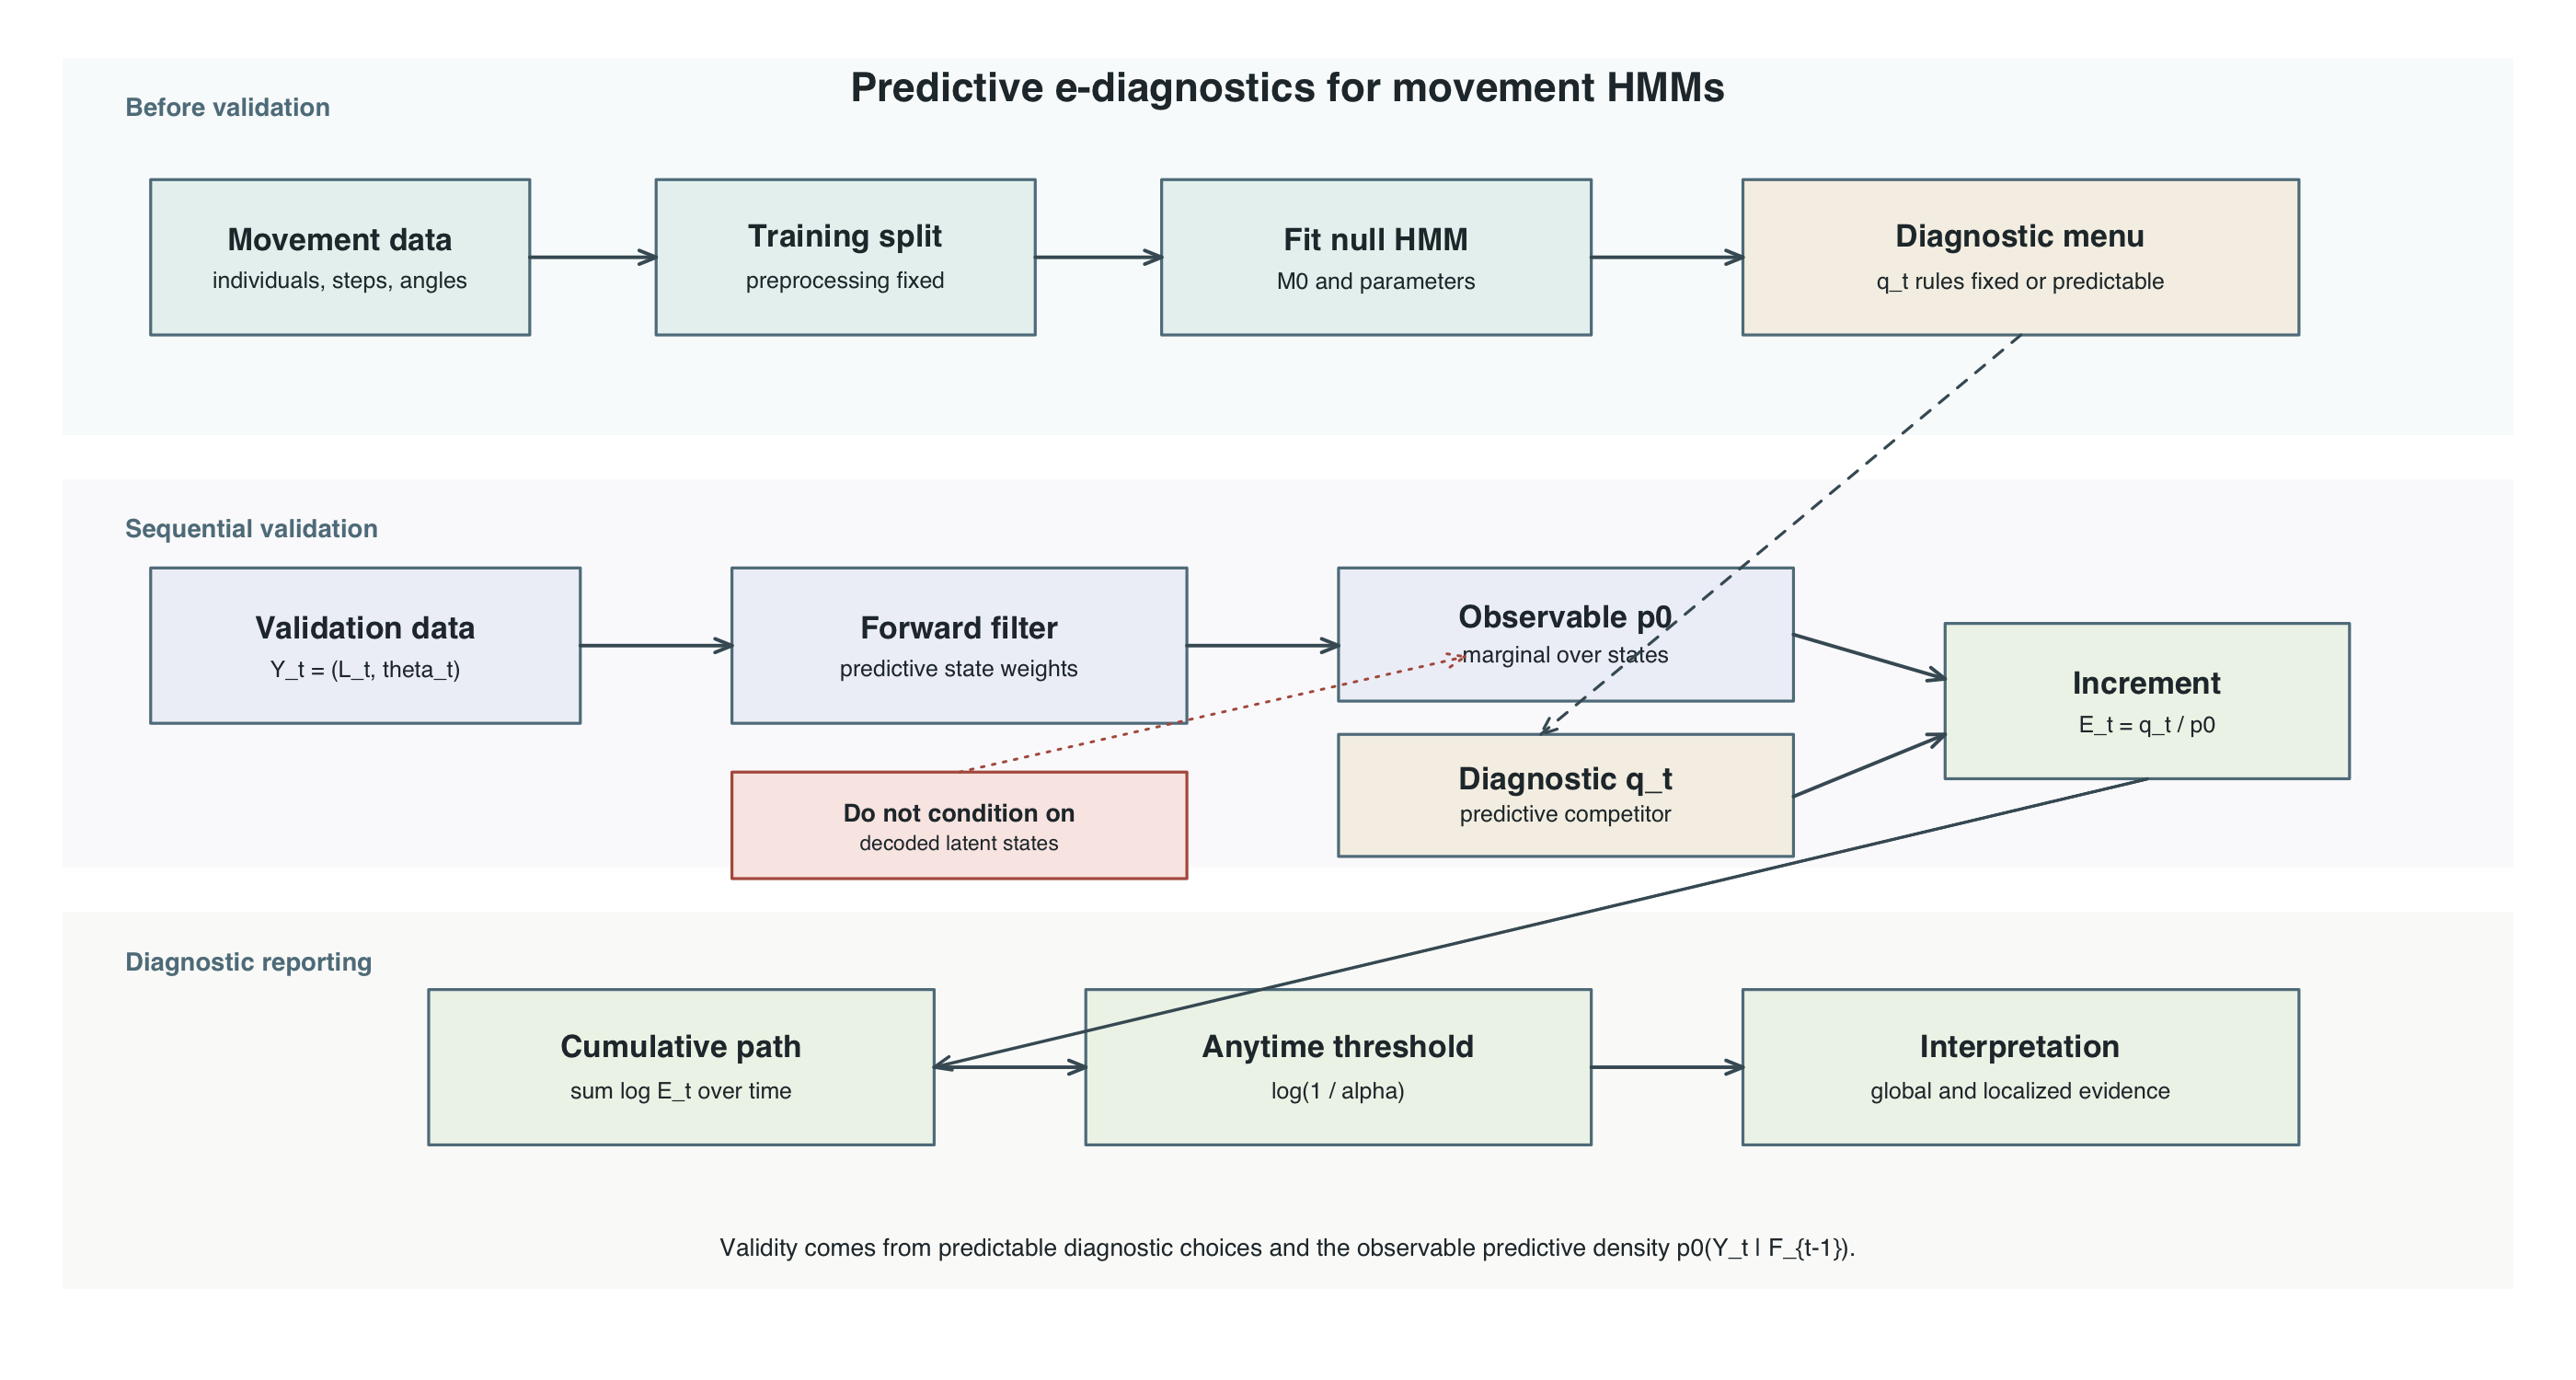
\includegraphics[width=\linewidth]{conceptual_workflow.png}
\caption{Conceptual workflow for predictive e-diagnostics. Training data determine the fitted null HMM, preprocessing choices and diagnostic menu before validation. During validation, the null denominator is the observable predictive density obtained by filtering over latent states. Diagnostic alternatives provide predictable competitors, density ratios produce e-value increments, and cumulative paths are reported through global, localized and threshold-crossing summaries.}
\label{fig:conceptual_workflow}
\end{figure}

\section{Validation protocol and movement HMM}
\label{sec:setup}

\subsection{Training information and validation filtration}

Let $(\Omega, \mathcal{A})$ be the underlying measurable space. Let $\calH \subseteq \mathcal{A}$ be the pre-validation sigma-field generated by the training data, fitted parameters, preprocessing choices, random seeds, and diagnostic-menu choices. All modelling choices in $\calH$ must be fixed before validation. Throughout, $\Pbb_0$ denotes the conditional validation law induced by the fitted generator after conditioning on $\calH$. Equivalently, all statements may be read under a regular conditional distribution $\Pbb_0(\cdot\mid\calH)$, with fitted parameters, diagnostic rules, and preprocessing fixed. Under this conditional validation law $\Pbb_0$, the validation sequence has one-step predictive density $p_0(y_t \mid \calF_{t-1})$. All e-process guarantees are conditional on $\calH$, and the unconditional guarantees follow by iterated expectation. This avoids any ambiguity about parameter uncertainty or whether the training data themselves are modeled.

The validation trajectory is indexed by $t=1,\ldots,T$. The observed movement variable is a measurable mapping $Y_t:\Omega \to \calY_t$ given by
\begin{equation}
Y_t=(L_t,\Theta_t),
\end{equation}
where $L_t$ is a step length and $\Theta_t$ is a turning angle. More generally, $Y_t$ may include several movement streams or covariates observed at the same temporal resolution. The latent behavioural state is
\begin{equation}
S_t\in\{1,\ldots,K\}.
\end{equation}
The observable validation filtration is defined as
\begin{equation}
\calF_t=\sigma(\calH,Y_1,\ldots,Y_t),\qquad t\geq 0,
\end{equation}
where $\calF_0=\calH$. To avoid measure-theoretic complications under composite nulls (since completing a filtration under one probability measure $\Pbb_\theta$ need not be complete under another), we do not complete the filtration, or when completion is formally required, we assume a universal completion under the family of candidate measures. Because our validation sequence is in discrete time, omitting completion is harmless and preserves mathematical validity. A diagnostic rule is called \emph{predictable} if the object used at time $t$ is $\calF_{t-1}$-measurable. Informally, predictable means that the diagnostic predictive alternative for $Y_t$ is chosen before $Y_t$ is revealed.

\begin{table}[t]
\centering
\begin{tabular}{>{\raggedright\arraybackslash}p{0.22\linewidth}>{\raggedright\arraybackslash}p{0.68\linewidth}}
\toprule
Notation & Meaning \\
\midrule
$Y_t$ & Observed movement variable at time $t$, often $(L_t,\Theta_t)$ \\
$L_t$ & Step length at time $t$ \\
$\Theta_t$ & Turning angle at time $t$ \\
$S_t$ & Latent behavioural state at time $t$ \\
$K$ & Number of states in the null HMM \\
$a_{1\mid 0}(s)$ & Initial predictive probability for state $s$ \\
$\calH$ & Training information fixed before validation \\
$\calF_t$ & Observable validation filtration, $\sigma(\calH,Y_1,\ldots,Y_t)$ \\
$M_0$ & Null HMM or fitted null generator \\
$p_0(y_t\mid\calF_{t-1})$ & Observable predictive density under $M_0$ \\
$q_t(y_t\mid\calF_{t-1})$ & Diagnostic predictive density or subdensity at time $t$ \\
$E_t$ & Predictive e-value increment at time $t$ \\
$E_{1:t}$ & Cumulative product of increments up to time $t$ \\
$\alpha$ & Anytime-valid monitoring level \\
\bottomrule
\end{tabular}
\caption{Notation used throughout the theoretical setup.}
\label{tab:notation}
\end{table}

\subsection{Null HMM}

Conditional on $\calH$, the null model $M_0$ is a fixed $K$-state HMM with initial distribution $\boldsymbol\pi_0$, transition matrix $\boldsymbol\Gamma_0$ and state-dependent observation densities. Let $X_t$ be the vector of covariates available at step $t$. Write
\begin{equation}
 f_{0,t,s}(y_t\mid X_t)=p_0(y_t\mid S_t=s, X_t)
\end{equation}
for the state-dependent density in state $s$. We explicitly assume that the covariates $X_t$ used to predict $Y_t$ are $\calF_{t-1}$-measurable, ensuring that the observation density processes are predictable. In movement ecology, this is a crucial distinction: environmental covariates evaluated at the animal's starting location at time $t-1$ (e.g., habitat class or temperature) are $\calF_{t-1}$-measurable and hence predictable. In contrast, covariates evaluated at the arrival location of step $t$ depend on the movement response $Y_t$ itself and are not predictable at time $t-1$, unless they are evaluated under the predicted step distribution. To simplify notation, covariates are suppressed below where clear, writing $f_{0,s}(y_t)$ or $f_{0,t,s}(y_t)$ as appropriate. In a common movement specification,
\begin{equation}
 f_{0,s}(l_t,\theta_t)=f^L_{0,s}(l_t)f^\Theta_{0,s}(\theta_t),
 \label{eq:conditional_independence}
\end{equation}
for example with Gamma step lengths and von Mises turning angles. The factorization in \eqref{eq:conditional_independence} is a modelling assumption, not a requirement of the e-process construction.

The HMM formulation also allows covariate-dependent transition probabilities, time-varying state-dependent parameters and multivariate observations, provided the one-step predictive density is well-defined and any covariates used to predict transitions $\Gamma_{0,t}(r,s)$ or observation densities are predictable.

\begin{table}[t]
\centering
\begin{tabular}{@{}>{\raggedright\arraybackslash}p{0.3\linewidth}>{\raggedright\arraybackslash}p{0.35\linewidth}>{\raggedright\arraybackslash}p{0.3\linewidth}@{}}
\toprule
Target & Validity claim & Practical interpretation \\
\midrule
Fixed fitted generator & Exact conditional e-process & ``Does this fitted HMM generate the validation trajectory?'' \\
True parametric HMM with estimated parameters & Not exact without adjustment & Requires parameter uncertainty treatment \\
Composite family & Uniform e-process via envelope or other safe construction & Conservative but genuine family-wise null \\
\bottomrule
\end{tabular}
\caption{Distinct statistical targets for movement model validation. This paper focuses primarily on the fixed fitted generator, treating the diagnostic as a check of the specific predictive model resulting from training.}
\label{tab:null_targets}
\end{table}

\section{Observable predictive density by filtering}
\label{sec:filtering}

The central object is the one-step-ahead observable predictive density. Since $S_t$ is latent, this density must marginalize over the predictive distribution of the state:
\begin{equation}
\label{eq:p0_predictive}
 p_0(y_t\mid \calF_{t-1})
  =\sum_{s=1}^K f_{0,t,s}(y_t\mid\calF_{t-1}^{\mathrm{cov}})\Pbb_0(S_t=s\mid \calF_{t-1}).
\end{equation}
This is the density of the next observed movement variable under the fitted HMM, conditional only on the observed past and the training information.

Let
\begin{equation}
 a_{t\mid t-1}(s)=\Pbb_0(S_t=s\mid \calF_{t-1})
\end{equation}
denote the predictive state probabilities before observing $Y_t$. This recursion must be explicitly initialized using the stationary or fitted initial distribution, $a_{1\mid 0}(s) = \pi_0(s)$. In applications with multiple validation individuals (such as cross-validation folds), the filter must be restarted for each held-out individual $i$ using $a_{i,1\mid 0}(s) = \pi_{0,i}(s)$. Then
\begin{equation}
 p_0(y_t\mid\calF_{t-1})=\sum_{s=1}^K a_{t\mid t-1}(s)f_{0,t,s}(y_t\mid\calF_{t-1}^{\mathrm{cov}}).
\end{equation}
After observing $Y_t=y_t$, the filtered probabilities are
\begin{equation}
\label{eq:filter_update}
 a_{t\mid t}(s)=\frac{a_{t\mid t-1}(s)f_{0,t,s}(y_t\mid\calF_{t-1}^{\mathrm{cov}})}{\sum_{r=1}^K a_{t\mid t-1}(r)f_{0,t,r}(y_t\mid\calF_{t-1}^{\mathrm{cov}})}.
\end{equation}
The next predictive state probabilities are
\begin{equation}
\label{eq:filter_predict}
 a_{t+1\mid t}(s)=\sum_{r=1}^K a_{t\mid t}(r)\Gamma_{0,t}(r,s),
\end{equation}
where $\Gamma_{0,t}(r,s) = \Pbb_0(S_{t+1}=s\mid S_t=r,\calF_t)$ defines the transition probability matrix convention. If transition probabilities depend on covariates, $\Gamma_{0,t}$ must be $\calF_t$-measurable (i.e., any covariates used for predicting $S_{t+1}$ must be known at time $t$). Crucially, spatial covariates computed from the animal's arrival location (such as habitat at the end of a step or distance to water after moving) are only predictable if they can be determined exactly from information available before observing $Y_t$, or if the diagnostic explicitly targets the joint distribution of the movement and the spatial context. The time-homogeneous HMM is the special case where $\Gamma_{0,t} \equiv \Gamma_0$, under which transitions are stationary. When transition probabilities depend on covariates, a stationary distribution generally does not exist, and the filter must be initialized using the fitted initial distribution $\pi_0$ or a pre-specified distribution.
Equations \eqref{eq:p0_predictive} to \eqref{eq:filter_predict} provide the computational basis of the null predictive density. They are also the reason the method differs from diagnostics based on Viterbi or other decoded state paths.

\section{Predictive e-values}
\label{sec:evalues}

\subsection{Diagnostic alternatives as predictable densities}

A diagnostic alternative is represented by a predictable Markov kernel or sub-Markov kernel $Q_t$. When represented by a density or subdensity $q_t(y\mid\calF_{t-1})$ with respect to a common dominating measure, the joint map $(\omega, y) \mapsto q_t(y\mid\calF_{t-1})(\omega)$ must be $\calF_{t-1} \otimes \calY$-measurable. The subscript $t$ allows the diagnostic to depend on the observed past. The key requirement is predictability: the rule defining $q_t$ must be fixed before observing $Y_t$.

Examples include:
\begin{itemize}[leftmargin=1.5em]
\item a $K+1$ state HMM used to diagnose whether the null HMM has too few states;
\item a more flexible angular distribution used to diagnose misspecified turning angles;
\item a joint step-angle model used to diagnose residual dependence between $L_t$ and $\Theta_t$ within behavioural states;
\item a duration-aware alternative, such as a hidden semi-Markov model (HSMM), used to diagnose non-geometric state dwell times;
\item a flexible predictive model trained on independent data and used as a diagnostic competitor to the fitted HMM.
\end{itemize}
These alternatives are diagnostic predictive competitors. They need not be interpreted as true data-generating mechanisms.

Throughout, all predictive distributions and diagnostic competitors are represented by densities with respect to a common dominating measure $\mu_t$ on the observation space at time $t$. This can be Lebesgue measure for continuous step-angle observations, counting measure for discrete observations or a product measure for mixed data. The convention is that ratios are evaluated only on the support of the null predictive density; outside that support the null event has probability zero, and we adopt the support convention that $q_t(y\mid\calF_{t-1}) = 0$ whenever $p_0(y\mid\calF_{t-1}) = 0$. Diagnostic competitors $q_t$ may be fixed before validation, or updated sequentially online using past validation observations, provided the update rule is predictable.

\begin{definition}[Predictive e-value increment]
For $t=1,\ldots,T$, define
\begin{equation}
\label{eq:increment}
 E_t=\frac{q_t(Y_t\mid\calF_{t-1})}{p_0(Y_t\mid\calF_{t-1})},
\end{equation}
whenever the ratio is well-defined under $M_0$.
\end{definition}

\begin{definition}[Predictive e-process]
The cumulative process is
\begin{equation}
\label{eq:eprocess}
 E_{1:t}=\prod_{u=1}^t E_u,
 \qquad E_{1:0}=1.
\end{equation}
Equivalently,
\begin{equation}
\label{eq:log_eprocess}
 \log E_{1:t}=\sum_{u=1}^t\left\{\log q_u(Y_u\mid\calF_{u-1})-\log p_0(Y_u\mid\calF_{u-1})\right\}.
\end{equation}
\end{definition}

\subsection{Main guarantee}

\begin{theorem}[Predictive e-process for a fixed HMM]
\label{thm:predictive_eprocess}
Assume that, conditional on $\calH$, the validation sequence is generated under the null HMM $M_0$, and that $p_0(y\mid\calF_{t-1})$ is the corresponding observable predictive density with respect to $\mu_t$. Let $q_t(y\mid\calF_{t-1})$ be an $\calF_{t-1}$-measurable diagnostic subdensity satisfying
\begin{equation}
 \int q_t(y\mid\calF_{t-1})\dd\mu_t(y)\leq 1
\end{equation}
almost surely. We assume either $q_t \ll p_0$ almost surely, or we define the ratio $E_t = 0$ on the set $\{y : p_0(y \mid \calF_{t-1}) = 0\}$ and evaluate the process under the validation law $\Pbb_0$. Under the latter convention, any diagnostic mass assigned outside the support of the null density is silently truncated. Then
\begin{equation}
 \E_0(E_t\mid\calF_{t-1})\leq 1.
\end{equation}
Consequently, $(E_{1:t})_{0\le t\le T}$ is a nonnegative supermartingale under $M_0$. If $q_t(\cdot\mid\calF_{t-1})$ is a density assigning all its mass to the support of $p_0(\cdot\mid\calF_{t-1})$, then equality holds and $(E_{1:t})_{0\le t\le T}$ is a martingale.
\end{theorem}

\begin{proof}
Conditional on $\calF_{t-1}$, $Y_t$ has density $p_0(y\mid\calF_{t-1})$ under $M_0$. Under the convention $E_t = 0$ on $\{p_0 = 0\}$, we have:
\begin{align}
\E_0(E_t\mid\calF_{t-1})
&=\int_{\{p_0>0\}}\frac{q_t(y\mid\calF_{t-1})}{p_0(y\mid\calF_{t-1})}p_0(y\mid\calF_{t-1})\dd\mu_t(y)\\
&=\int_{\{p_0>0\}}q_t(y\mid\calF_{t-1})\dd\mu_t(y)\\
&\leq 1.
\end{align}
Note that defining $E_t = 0$ on $\{p_0 = 0\}$ truncates any diagnostic mass assigned outside the null support. While this preserves e-process validity, it ignores discrepancies on null-impossible events. For the cumulative process,
\begin{align}
\E_0(E_{1:t}\mid\calF_{t-1})
&=E_{1:t-1}\E_0(E_t\mid\calF_{t-1})\\
&\leq E_{1:t-1}.
\end{align}
Thus $(E_{1:t})_{0\le t\le T}$ is a nonnegative supermartingale. If $q_t$ is a density supported by the null support, the conditional expectation is one at every time, giving the martingale case.
\end{proof}

\begin{corollary}[Optional stopping and anytime-valid monitoring]
\label{cor:optional_stopping}
Under the conditions of Theorem \ref{thm:predictive_eprocess}, for any $\alpha\in(0,1)$,
\begin{equation}
 \Pbb_0\left(\sup_{0\leq t\leq T}E_{1:t}\geq \frac{1}{\alpha}\right)\leq \alpha.
\end{equation}
Equivalently,
\begin{equation}
 \Pbb_0\left(\sup_{0\leq t\leq T}\log E_{1:t}\geq \log(1/\alpha)\right)\leq \alpha.
\end{equation}
Moreover, for any stopping time $\tau$ with respect to $(\calF_t)$, the stopped process $E_{1:\tau\wedge T}$ is an e-value under $M_0$, meaning $\E_0(E_{1:\tau\wedge T})\leq1$.
\end{corollary}

\noindent The proof is given in the supplementary material.

\begin{corollary}[Anytime p-value induced by an e-process]
\label{cor:anytime_p}
Define
\begin{equation}
 p_t^\mathrm{any}=\min\left\{1,\frac{1}{\sup_{0\leq u\leq t}E_{1:u}}\right\}.
\end{equation}
Then $p_t^\mathrm{any}$ is an anytime-valid p-value process in the sense that, under $M_0$,
\begin{equation}
 \Pbb_0\left(\exists \, 0 \le t \le T: p_t^\mathrm{any}\leq\alpha\right)\leq\alpha.
\end{equation}
\end{corollary}

\noindent The proof is given in the supplementary material.

\section{Why filtering is essential}
\label{sec:filtering_essential}

The proof of Theorem \ref{thm:predictive_eprocess} uses only one fact about the null model: the denominator must be the true conditional density of the next observable variable given the observable past. In an HMM, that density is not obtained by conditioning on a decoded state. It is obtained by marginalizing over the predictive state distribution.

\begin{proposition}[Validity is based on marginal observable prediction]
\label{prop:latent_filtering}
For an HMM, the denominator in \eqref{eq:increment} is the marginal observable predictive density
\begin{equation}
\label{eq:marginal_prediction}
 p_0(y_t\mid\calF_{t-1})=\sum_{s=1}^K f_{0,s}(y_t)\Pbb_0(S_t=s\mid\calF_{t-1}).
\end{equation}
The e-process validity does not require observing $S_t$ and does not generally follow from replacing $S_t$ by a decoded path $\widehat S_t$.
\end{proposition}

\begin{proof}
The proof of Theorem \ref{thm:predictive_eprocess} requires the denominator to be the conditional density of $Y_t$ given $\calF_{t-1}$. In an HMM this conditional law is obtained by summing over the unobserved state $S_t$ using the predictive state probabilities. A decoded path $\widehat S_t$ is a statistic produced by a fitted model and observed data. It does not appear in the conditional law of $Y_t$ given $\calF_{t-1}$ unless the decoded state is known to equal the true latent state, which is not the usual HMM setting.
\end{proof}

\begin{example}[A state-conditioned denominator can violate e-validity]
\label{ex:decoded_invalid}
Consider a two-state model at a single validation time with predictive state probabilities $1/2$ and $1/2$. Let
\[
 f_1(y)=\phi(y;-m,1),\qquad f_2(y)=\phi(y;m,1),
\]
where $\phi(\cdot;\mu,1)$ is the $N(\mu,1)$ density and $m>0$. The observable null density is
\[
 p_0(y)=\frac12 f_1(y)+\frac12 f_2(y).
\]
Suppose one incorrectly uses $f_1(y)$ as the denominator because a decoded or assigned state is set to state 1, and suppose the diagnostic numerator is $q(y)=f_2(y)$. The expected ratio under the true observable null is
\begin{align}
 \E_0\left\{\frac{f_2(Y)}{f_1(Y)}\right\}
 &=\int \frac{f_2(y)}{f_1(y)}\left\{\frac12f_1(y)+\frac12f_2(y)\right\}\dd y\\
 &=\frac12+\frac12\int\frac{f_2(y)^2}{f_1(y)}\dd y\\
 &=\frac12+\frac12\exp(4m^2),
\end{align}
which is larger than 1. Thus the ratio is not an e-value under the observable null. The problem is not the use of likelihood ratios; the problem is the use of the wrong denominator. This issue persists for data-dependent decoded states. Specifically, let $S'_t = s(Y_{1:t})$ be any state assignment mapping the validation path to a state (such as Viterbi path decoding or local state decoding). If one uses the state-conditioned density $f_{0,S'_t}(Y_t \mid \calF_{t-1})$ as the denominator, it is not predictable with respect to $\calF_{t-1}$ because it depends on the current observation $Y_t$ through $S'_t$. The expected ratio under the true null distribution satisfies
\begin{equation}
 \E_0\left\{ \frac{q_t(Y_t\mid\calF_{t-1})}{f_{0,S'_t}(Y_t\mid\calF_{t-1})} \;\middle|\; \calF_{t-1} \right\} \neq \int q_t(y\mid\calF_{t-1})\dd\mu_t(y),
\end{equation}
and is not bounded by 1 in general, violating e-validity. The denominator must always be the filtered marginal predictive density $p_0(Y_t \mid \calF_{t-1})$.
\end{example}

In movement terms, replacing the filtering mixture by a Viterbi state-specific turning-angle density can turn a descriptive behavioural state label into an invalid predictive denominator.

\begin{remark}[Decoded states are useful after, not before, validation]
A Viterbi path, local decoding or posterior state classification may be useful for interpretation after a diagnostic signal has been found. For example, one may report whether large local log-increments occur during times with high smoothed probability of a particular behaviour. Such summaries are descriptive unless the weights used for localization are predictable. Section \ref{sec:localization} gives a valid predictable alternative based on filtered state probabilities.
\end{remark}

\section{Predictable diagnostic selection, mixtures and parallel diagnostics}
\label{sec:mixtures}

In practice, the analyst may not want to commit to a single diagnostic alternative. One may want to compare a $K+1$ state HMM, an angular alternative, a copula alternative and a duration alternative. E-values are convenient here, but care is needed. Predictable switching, mixtures and sequential diagnostic workflows are valid when each new step is conditionally valid given the information already revealed. Products of parallel diagnostics computed on the same validation observations are not automatically valid.

\begin{proposition}[Predictable mixtures of diagnostic alternatives]
\label{prop:mixtures}
Let $q_{j,t}(y\mid\calF_{t-1})$, $j=1,\ldots,J$, be predictable diagnostic subdensities satisfying
\[
 \int q_{j,t}(y\mid\calF_{t-1})\mu_t(\mathrm dy)\leq1.
\]
Let $w_{j,t}\geq0$ be predictable weights with $\sum_{j=1}^Jw_{j,t}\leq1$. Define
\begin{equation}
 q_t^{\mathrm{mix}}(y\mid\calF_{t-1})=\sum_{j=1}^Jw_{j,t}q_{j,t}(y\mid\calF_{t-1})
\end{equation}
and
\begin{equation}
 E_t^{\mathrm{mix}}=\frac{q_t^{\mathrm{mix}}(Y_t\mid\calF_{t-1})}{p_0(Y_t\mid\calF_{t-1})}.
\end{equation}
Then $E_t^{\mathrm{mix}}$ is a conditional e-value increment, and $\prod_{u\leq t}E_u^{\mathrm{mix}}$ is an e-process under $M_0$.
\end{proposition}

\noindent The proof is given in the supplementary material.

\begin{corollary}[Predictable switching]
\label{cor:switching}
Let $J_t\in\{1,\ldots,J\}$ be $\calF_{t-1}$-measurable. Then
\begin{equation}
 E_t^{\mathrm{switch}}=\frac{q_{J_t,t}(Y_t\mid\calF_{t-1})}{p_0(Y_t\mid\calF_{t-1})}
\end{equation}
is a conditional e-value increment. Thus the analyst may switch among a pre-specified menu of diagnostic alternatives using only information available before the next validation observation.
\end{corollary}

\noindent The proof is given in the supplementary material.

\begin{proposition}[Sequential exploratory diagnostic workflows]
\label{prop:sequential_workflow}
Let $(\calG_j)_{j\geq0}$ be a filtration describing the information available after successive diagnostic stages, with $\calG_0$ containing the training information and any pre-validation design choices. Suppose that, at stage $j$, the analyst chooses a diagnostic rule using only $\calG_{j-1}$ and obtains a nonnegative random variable $D_j$ satisfying
\begin{equation}
 \E_0(D_j\mid\calG_{j-1})\leq1.
\end{equation}
Then
\begin{equation}
 D_{1:m}=\prod_{j=1}^m D_j,\qquad D_{1:0}=1,
\end{equation}
is a nonnegative supermartingale with respect to $(\calG_j)_{j\geq0}$. In particular,
\begin{equation}
 \Pbb_0\left(\sup_{0\leq m\leq M}D_{1:m}\geq\frac{1}{\alpha}\right)\leq\alpha
\end{equation}
for any finite number of stages $M$.
\end{proposition}

\noindent The proof is given in the supplementary material.

\begin{remark}[Exploratory diagnostics as conditional bets]
Proposition \ref{prop:sequential_workflow} formalizes a controlled version of exploratory model criticism. After seeing one diagnostic, the analyst may decide which diagnostic to run next, which segment to inspect, or which fresh validation unit to use, provided the next diagnostic e-value is valid conditionally on all information revealed so far. The result does not justify multiplying several diagnostic outputs that were computed in parallel on the same observations after inspecting them; that setting is covered by Proposition \ref{prop:parallel}.
\end{remark}

\begin{proposition}[Parallel diagnostics on the same validation data]
\label{prop:parallel}
Suppose $E^{(1)},\ldots,E^{(J)}$ are e-values under $M_0$ computed from the same validation experiment, so that $\E_0E^{(j)}\leq1$ for each $j$. If $w_j\geq0$ and $\sum_jw_j\leq1$, then
\begin{equation}
 E^{\mathrm{avg}}=\sum_{j=1}^Jw_jE^{(j)}
\end{equation}
is also an e-value under $M_0$. Consequently,
\begin{equation}
 \Pbb_0\left(\max_{1\leq j\leq J}w_jE^{(j)}\geq \frac{1}{\alpha}\right)\leq\alpha.
\end{equation}
In contrast, the product $\prod_{j=1}^JE^{(j)}$ is not generally an e-value when the diagnostics are computed in parallel on the same observations.
\end{proposition}

\noindent The proof is given in the supplementary material.

\begin{remark}[Recommended reporting for several diagnostics]
For a diagnostic menu evaluated on the same validation sequence, report the individual e-processes and either use a weighted average e-value or pre-assigned weighted thresholds. A product of diagnostic e-processes is valid only when the factors are accumulated as a sequential process with each new factor conditionally valid given all previous diagnostic outcomes and using the appropriate next unit of information.
\end{remark}

\section{Localization, state weighting and tempering}
\label{sec:localization}

A global e-process answers whether a diagnostic alternative accumulates evidence against the null generator. Movement ecologists usually also want to know where the failure occurs: during migration, in a given habitat, for one individual, or during time periods in which the fitted model predicts a particular behavioural state. The following result gives a valid way to localize evidence when the localization weights are predictable.

\begin{proposition}[Predictable weighted localization]
\label{prop:weighted_localization}
Let $E_t$ be any conditional e-value increment satisfying $\E_0(E_t\mid\calF_{t-1})\leq1$. Let $W_t$ be any $\calF_{t-1}$-measurable weight with $0\leq W_t\leq1$. Define
\begin{equation}
\label{eq:weighted_increment}
 E_t^{(W)}=1+W_t(E_t-1).
\end{equation}
Then $E_t^{(W)}\geq0$ and
\begin{equation}
 \E_0(E_t^{(W)}\mid\calF_{t-1})\leq1.
\end{equation}
Consequently, $\prod_{u\leq t}E_u^{(W)}$ is an e-process under $M_0$.
\end{proposition}

\noindent The proof is given in the supplementary material.

\begin{corollary}[Segment-specific e-processes]
\label{cor:segment}
If $B_t$ is a predictable indicator of a biologically meaningful segment, such as a known season, a habitat class known before observing the movement response, or a held-out individual, then
\begin{equation}
 E_t^{(B)}=\begin{cases}
 E_t, & B_t=1,\\
 1, & B_t=0,
 \end{cases}
\end{equation}
yields a valid segment-specific e-process. Thus evidence can be accumulated only over a pre-specified or predictably selected subset of times.
\end{corollary}

\noindent The proof is given in the supplementary material.

\begin{corollary}[Soft state-localized e-processes]
\label{cor:state_localized}
For a fitted HMM, set
\begin{equation}
 W_t^{(s)}=a_{t\mid t-1}(s)=\Pbb_0(S_t=s\mid\calF_{t-1}).
\end{equation}
Then
\begin{equation}
 E_t^{(s)}=1+a_{t\mid t-1}(s)(E_t-1)
\end{equation}
defines a valid e-process localized to times at which state $s$ is predicted to be likely under the null model.
\end{corollary}

\noindent The proof is given in the supplementary material.

\begin{proposition}[Power-tempered and linearly tempered e-increments]
\label{prop:tempering}
Let $E_t$ be a conditional e-value increment. If $\lambda_t\in[0,1]$ is predictable, then both
\begin{equation}
 \widetilde E_t^{\mathrm{pow}}=E_t^{\lambda_t}
\end{equation}
(with the convention $0^0=1$) and
\begin{equation}
 \widetilde E_t^{\mathrm{lin}}=1+\lambda_t(E_t-1)
\end{equation}
are conditional e-value increments. Their products are e-processes.
\end{proposition}

\noindent The proof is given in the supplementary material.

\begin{remark}[Interpretation of localized evidence]
The process in Corollary \ref{cor:state_localized} is not the same as conditioning on the event that the true latent state equals $s$. It is a valid soft localization based on the null model's predictive probability of state $s$. Smoothed state probabilities using future observations can be useful for visualization, but they are not predictable and therefore do not by themselves preserve the e-process guarantee.
\end{remark}

\section{Feature-level and blockwise e-diagnostics}
\label{sec:feature_block}

The previous sections use full predictive densities for $Y_t$. In movement applications, the diagnostically relevant object may be a lower-dimensional feature, such as a circular residual, a transformed step length, a copula residual, a barrier-crossing indicator or a blockwise spatial statistic. E-values can be constructed directly from such features if their null conditional law is known.

\begin{theorem}[Feature-level predictive e-values]
\label{thm:feature}
Let $Z_t=\psi_t(Y_t,\calF_{t-1})$ be a diagnostic feature whose transformation rule $\psi_t$ is predictable. Let $g_{0,t}(z\mid\calF_{t-1})$ be the conditional density of $Z_t$ under $M_0$, and let $g_{1,t}(z\mid\calF_{t-1})$ be a predictable diagnostic subdensity satisfying $\int g_{1,t}(z\mid\calF_{t-1})\nu_t(\mathrm dz)\leq1$. Define
\begin{equation}
 R_t=\frac{g_{1,t}(Z_t\mid\calF_{t-1})}{g_{0,t}(Z_t\mid\calF_{t-1})}.
\end{equation}
Then $R_t$ is a conditional e-value increment under $M_0$, and $\prod_{u\leq t}R_u$ is an e-process.
\end{theorem}

\begin{proof}
Conditional on $\calF_{t-1}$, $Z_t$ has density $g_{0,t}(z\mid\calF_{t-1})$ under $M_0$. Therefore,
\[
 \E_0(R_t\mid\calF_{t-1})=\int_{\{g_0>0\}}g_{1,t}(z\mid\calF_{t-1})\nu_t(\mathrm dz)\leq1.
\]
The product result follows as before.
\end{proof}

\begin{remark}[Discrete and mixed features]
The feature-level theorem holds for any dominating measure $\nu_t$. If $Z_t$ is discrete (such as a count of barrier crossings or state transitions within a block), $g_{0,t}$ and $g_{1,t}$ are probability mass functions, and $\nu_t$ is the counting measure. For discrete features, standard probability integral transforms (PIT) are not uniform, but one can use randomized PITs to obtain uniform continuous residuals, or work directly with the discrete probability mass functions in the density-ratio increment $R_t$.
\end{remark}

\subsection{Rosenblatt residuals and step-angle dependence}

Feature-level e-values are especially useful for circular-linear diagnostics. Suppose the null model gives a joint predictive distribution for $Y_t=(L_t,\Theta_t)$. A sequential Rosenblatt transform can be defined by
\begin{align}
 U_t^L &= F_{0,t}^L(L_t\mid\calF_{t-1}),\\
 U_t^\Theta &= F_{0,t}^{\Theta\mid L}(\Theta_t\mid L_t,\calF_{t-1}),
\end{align}
where the second conditional distribution respects the circular support of $\Theta_t$. Crucially, $F_{0,t}^L$ and $F_{0,t}^{\Theta\mid L}$ are cumulative distribution functions derived from the marginal observable predictive mixture $p_0(y_t\mid\calF_{t-1})$ (by marginalizing over the latent states using filtered probabilities), not from a decoded state or state-conditioned distribution. Under a continuous correctly specified null predictive distribution, $(U_t^L,U_t^\Theta)$ is conditionally uniform on $[0,1]^2$. A copula diagnostic can therefore use
\begin{equation}
 R_t^{\mathrm{cop}}=c_\rho(U_t^L,U_t^\Theta),
\end{equation}
where $c_\rho$ is a copula density on $[0,1]^2$, with $\rho$ fixed from training or chosen predictably. Theorem \ref{thm:feature} gives conditional e-validity because $c_\rho$ integrates to one under the uniform null. This construction targets residual step-angle dependence after the fitted HMM has already accounted for latent behavioural states.

\begin{remark}[Circular data]
Turning angles live on the circle, so residual diagnostics should respect periodicity. One may work with circular distribution functions relative to a chosen origin, with probability integral transforms for von Mises or mixture von Mises predictive distributions, or with features such as $\cos(\Theta_t-\mu_t)$ whose null law is derived from the circular predictive distribution. The e-value requirement is not normality of residuals; it is knowledge or independent estimation of the feature's null predictive law.
\end{remark}

\subsection{Blockwise diagnostics for long-horizon movement summaries}

One-step predictive diagnostics are local. Movement-model failures can also appear only over longer horizons, for example through utilization distributions, mean squared displacement, straightness, return times, residence times or barrier crossing frequencies. These can be handled by blockwise e-values.

\begin{theorem}[Blockwise predictive e-values for predictable boundaries]
\label{thm:block_predictable}
Let $0=\tau_0<\tau_1<\tau_2<\cdots$ be stopping times such that each block length $T_j = \tau_j - \tau_{j-1}$ is $\calF_{\tau_{j-1}}$-measurable. This includes deterministic block boundaries (e.g., daily, weekly, or seasonal blocks). For block $j$, write $Y_{B_j}=Y_{\tau_{j-1}+1:\tau_j}$. Let $p_{0,j}(y_{B_j}\mid\calF_{\tau_{j-1}}) = \prod_{t=\tau_{j-1}+1}^{\tau_j} p_0(y_t\mid\calF_{t-1})$ be the conditional null predictive density of the block, and let $q_j(y_{B_j}\mid\calF_{\tau_{j-1}})$ be a predictable diagnostic subdensity on $\calY^{T_j}$. Define
\begin{equation}
 E_j^{\mathrm{block}}=\frac{q_j(Y_{B_j}\mid\calF_{\tau_{j-1}})}{p_{0,j}(Y_{B_j}\mid\calF_{\tau_{j-1}})}.
\end{equation}
Then $(\prod_{r\leq j}E_r^{\mathrm{block}})_{j\geq0}$ is an e-process under $M_0$.
\end{theorem}

\begin{proof}
Conditional on $\calF_{\tau_{j-1}}$, the block $Y_{B_j}$ has density $p_{0,j}$ under $M_0$ and the length $T_j$ is fixed. Since $q_j$ is a subdensity on $\calY^{T_j}$, the same density-ratio calculation as in Theorem \ref{thm:predictive_eprocess} gives $\E_0(E_j^{\mathrm{block}}\mid\calF_{\tau_{j-1}})\leq1$. The cumulative product over blocks is therefore a nonnegative supermartingale with respect to the block filtration $(\calF_{\tau_j})_{j\geq 0}$.
\end{proof}

\begin{theorem}[Blockwise e-values for genuinely stopped blocks]
\label{thm:block_stopped}
Suppose the block boundary $\tau_j$ is a stopping time that depends on observations inside the block (e.g., stopping when the animal leaves a home range or crosses a spatial boundary). Let the stopped block variable be $X_j = (Y_{B_j}, M_j)$, where $M_j = \tau_j - \tau_{j-1}$ is the random block length. Under $M_0$, the conditional joint density of the path $y_{1:m}$ and stopping event $M_j = m$ is:
\begin{equation}
 p_{0,j}(y_{1:m}, m\mid\calF_{\tau_{j-1}}) = \left( \prod_{t=\tau_{j-1}+1}^{\tau_{j-1}+m} p_0(y_t\mid\calF_{t-1}) \right) \Pbb_0(\tau_j - \tau_{j-1} = m \mid Y_{\tau_{j-1}+1:\tau_{j-1}+m} = y_{1:m}, \calF_{\tau_{j-1}}).
\end{equation}
Let $q_j(y_{1:m}, m \mid \calF_{\tau_{j-1}})$ be a predictable diagnostic subdensity on the variable-length space $\bigcup_{m=1}^\infty (\calY^m \times \{m\})$. Define
\begin{equation}
 E_j^{\mathrm{block}}=\frac{q_j(Y_{B_j}, M_j\mid\calF_{\tau_{j-1}})}{p_{0,j}(Y_{B_j}, M_j\mid\calF_{\tau_{j-1}})}.
\end{equation}
Then $(\prod_{r\leq j}E_r^{\mathrm{block}})_{j\geq0}$ is an e-process under $M_0$.
\end{theorem}

\begin{proof}
Conditional on $\calF_{\tau_{j-1}}$, the random variable $X_j$ has joint density $p_{0,j}$ with respect to the product of the dominating measure on $\calY^m$ and the counting measure on $\mathbb{N}^+$. Since $q_j$ is a subdensity on the Stopped-Path space, we have:
\begin{align}
 \E_0(E_j^{\mathrm{block}}\mid\calF_{\tau_{j-1}})
 &= \sum_{m=1}^\infty \int \frac{q_j(y_{1:m}, m \mid \calF_{\tau_{j-1}})}{p_{0,j}(y_{1:m}, m \mid \calF_{\tau_{j-1}})} p_{0,j}(y_{1:m}, m \mid \calF_{\tau_{j-1}}) \dd\mu^{(m)}(y_{1:m}) \\
 &= \sum_{m=1}^\infty \int q_j(y_{1:m}, m \mid \calF_{\tau_{j-1}}) \dd\mu^{(m)}(y_{1:m}) \leq 1.
\end{align}
The cumulative product over blocks is therefore a nonnegative supermartingale with respect to $(\calF_{\tau_j})_{j\geq 0}$.
\end{proof}

\begin{corollary}[Feature-level block diagnostics]
\label{cor:block_feature}
Let $Z_j=h_j(Y_{B_j},\calF_{\tau_{j-1}})$ be a predictable block feature such as a barrier-crossing indicator, a displacement statistic or a summary of space use over the block. If the conditional null density or mass function of $Z_j$ is $g_{0,j}$ and a diagnostic alternative is $g_{1,j}$, then $g_{1,j}(Z_j)/g_{0,j}(Z_j)$ is a blockwise e-value increment.
\end{corollary}

\begin{proof}
Apply Theorem \ref{thm:feature} at the block level.
\end{proof}

\begin{remark}[Simulation-based block laws]
When the null law of a block feature is unavailable analytically, it may be approximated by simulation from the fitted HMM using only training information and the observed block covariates. Exact finite-sample e-validity then depends on how the density or mass estimate is constructed. A conservative recommendation for a first implementation is to fit any feature-level diagnostic law on independent null simulations or training data, and to reserve a separate validation trajectory for the final e-process calculation.
\end{remark}

\section{Estimated parameters, split validation and composite nulls}
\label{sec:estimated}

The exact theory above treats $M_0$ as a fixed generator at validation time. In applied movement modelling, $M_0$ is fitted. This section separates three interpretations: conditional validity for a fitted generator, cross-fitted e-values over independent validation units and conservative composite-null envelopes.

\subsection{Conditional validity after training}

\begin{theorem}[Split-sample conditional validity]
\label{thm:split}
Let $\calH$ contain the training data and all fitted parameters of the null and diagnostic alternatives. Suppose that, conditional on $\calH$, the validation trajectory is generated from the fitted null predictive law $p_0(\cdot\mid\calF_{t-1})$, and suppose $q_t$ is predictable with respect to $\calF_{t-1}=\calH\vee\sigma(Y_1,\ldots,Y_{t-1})$. Then the process in Theorem \ref{thm:predictive_eprocess} is an e-process conditional on $\calH$. In particular,
\begin{equation}
 \Pbb_0\left(\sup_{0 \le t \le T}E_{1:t}\geq1/\alpha\mid\calH\right)\leq\alpha
\end{equation}
almost surely, and the same bound holds unconditionally.
\end{theorem}

\noindent The proof is given in the supplementary material.

This theorem clarifies the interpretation of the first article's target: the exact null is that the held-out validation sequence is generated by the fitted HMM. It is a diagnostic check of the fitted generator, not a claim that the parameter estimator has no uncertainty.

\subsection{Independent validation units and cross-fitted averages}

A natural movement design trains on some individuals and validates on held-out individuals. If each held-out individual yields an e-value, these e-values can be reported individually or combined by averaging.

\begin{proposition}[Cross-fitted average over validation units]
\label{prop:crossfit_average}
Suppose $E^{(i)}$ is an e-value under $M_0$ for validation unit $i$, for $i=1,\ldots,n$, where each $E^{(i)}$ may be constructed using a model fitted on data not including the validation responses of unit $i$. If $w_i\geq0$ and $\sum_iw_i\leq1$, then
\begin{equation}
 E^{\mathrm{cf}}=\sum_{i=1}^nw_iE^{(i)}
\end{equation}
is an e-value under $M_0$.
\end{proposition}

\noindent The proof is given in the supplementary material.
\begin{remark}[Leave-one-individual-out products and joint nulls]
A leave-one-individual-out workflow may produce individually valid e-values, but the product across individuals is not automatically valid because the fitted models may use overlapping training sets and the e-values are computed in parallel. Specifically, conditional on the training set for fold $i$, $E^{(i)}$ is valid for the hypothetical validation law generated by the fold-specific fitted model. The average $E^{\mathrm{cf}}$ is valid if all fold-specific validation laws are embedded in a common joint null under which each $E^{(i)}$ has expectation at most one. Alternatively, leave-one-animal-out (LOAO) cross-validation should be presented as a practical cross-predictive diagnostic rather than an exact global test, unless a coherent joint null is specified. The weighted average in Proposition \ref{prop:crossfit_average} is a safer default unless a sequential data-collection or sample-splitting design is used.
\end{remark}

\subsection{A conservative envelope for composite null families}
\label{sec:envelope}

The fitted-generator null is often the most transparent target for model criticism. If one instead wants a single process valid for every parameter value in a null family, a conservative envelope construction is possible.

\begin{proposition}[Composite-null envelope]
\label{prop:envelope}
Let $\{p_\theta(y\mid\calF_{t-1}):\theta\in\Theta_0\}$ be a family of null predictive densities. Assume that the pointwise supremum
\begin{equation}
 p_t^{\mathrm{env}}(y\mid\calF_{t-1})=\sup_{\theta\in\Theta_0}p_\theta(y\mid\calF_{t-1})
\end{equation}
is measurable, positive wherever any $p_\theta$ is positive, and finite on the relevant support. This is typically satisfied if $\Theta_0$ is a finite family, or by using an essential supremum over a well-controlled parametric family. Let $q_t$ be a predictable diagnostic subdensity. Define
\begin{equation}
 \overline E_t=\frac{q_t(Y_t\mid\calF_{t-1})}{p_t^{\mathrm{env}}(Y_t\mid\calF_{t-1})}.
\end{equation}
Then for every $\theta\in\Theta_0$,
\begin{equation}
 \E_\theta(\overline E_t\mid\calF_{t-1})\leq1,
\end{equation}
and $\prod_{u\leq t}\overline E_u$ is an e-process uniformly valid over the composite null family.
\end{proposition}

\noindent The proof is given in the supplementary material.

\begin{remark}[Cost and limits of envelope validity]
The envelope denominator is usually not a density and may be much larger than any single fitted predictive density. The resulting e-process can be conservative and computationally difficult for HMMs. Moreover, continuous envelopes over unrestricted Gamma or von Mises families may be infinite, unstable, or computationally prohibitive. The envelope construction is therefore primarily practical for finite or compactly restricted parameter families, rather than general HMM parameter spaces.
\end{remark}

\section{Behaviour under misspecification}
\label{sec:power}

The e-process guarantee controls false alarms under the null. Its usefulness under alternatives depends on the diagnostic bet. The following results connect e-process growth to prequential log-score differences.

\begin{proposition}[Conditional log-score decomposition]
\label{prop:kl_decomposition}
Let $p_\star(\cdot\mid\calF_{t-1})$ be the true conditional density of $Y_t$ under a data-generating process $P_\star$. Let $q_t$ and $p_0$ be predictive densities. If the relevant integrals are finite, then
\begin{align}
 \E_\star\left[\log\frac{q_t(Y_t\mid\calF_{t-1})}{p_0(Y_t\mid\calF_{t-1})}\middle|\calF_{t-1}\right]
 &=\KL\{p_\star(\cdot\mid\calF_{t-1}),p_0(\cdot\mid\calF_{t-1})\}\\
 &\quad -\KL\{p_\star(\cdot\mid\calF_{t-1}),q_t(\cdot\mid\calF_{t-1})\}.
\end{align}
Thus the expected local log-increment is positive exactly when the diagnostic alternative is closer than the null in conditional Kullback-Leibler risk.
\end{proposition}

\begin{proof}
By definition,
\begin{align}
\E_\star\left[\log\frac{q_t(Y_t\mid\calF_{t-1})}{p_0(Y_t\mid\calF_{t-1})}\middle|\calF_{t-1}\right]
&=\int p_\star(y\mid\calF_{t-1})\log\frac{q_t(y\mid\calF_{t-1})}{p_0(y\mid\calF_{t-1})}\mu_t(\mathrm dy)\\
&=\int p_\star\log\frac{p_\star}{p_0}\mu_t(\mathrm dy)-\int p_\star\log\frac{p_\star}{q_t}\mu_t(\mathrm dy),
\end{align}
which is the displayed identity.
\end{proof}

\begin{proposition}[Asymptotic growth under positive drift]
\label{prop:growth}
Let $X_t=\log E_t$ and suppose under $P_\star$ that
\begin{equation}
 \delta_t=\E_\star(X_t\mid\calF_{t-1})
\end{equation}
exists. Assume the martingale differences $X_t-\delta_t$ satisfy a strong law, for example
\begin{equation}
 \frac{1}{T}\sum_{t=1}^T\{X_t-\delta_t\}\to0\qquad P_\star\text{-a.s.}
\end{equation}
If
\begin{equation}
 \frac{1}{T}\sum_{t=1}^T\delta_t\to\delta>0,
\end{equation}
then
\begin{equation}
 \frac{1}{T}\log E_{1:T}\to\delta\qquad P_\star\text{-a.s.}
\end{equation}
In particular, the e-process grows exponentially at asymptotic rate $\delta$.
\end{proposition}

\begin{proof}
Using $\log E_{1:T}=\sum_{t=1}^TX_t$,
\begin{equation}
 \frac{1}{T}\log E_{1:T}=\frac{1}{T}\sum_{t=1}^T\delta_t+\frac{1}{T}\sum_{t=1}^T(X_t-\delta_t).
\end{equation}
The first term converges to $\delta$ by assumption and the second to zero by the assumed martingale strong law.
\end{proof}

\begin{remark}[Power is diagnostic-specific]
A large e-process is evidence against the null relative to the alternative used to construct the diagnostic. If the null HMM has an ecologically important defect but the alternative does not predict that defect better, the e-process may not grow. This is a feature rather than a failure: the method localizes model criticism through explicit diagnostic predictive alternatives.
\end{remark}

\section{Movement-specific diagnostic catalogue}
\label{sec:catalogue}

Table \ref{tab:diagnostics} summarizes a practical menu of diagnostics. Each diagnostic can be implemented as a full predictive density ratio, a feature-level e-value, or a blockwise e-value depending on the available null law and the scientific target.

\begin{table}[t]
\centering
\footnotesize
\begin{tabular}{@{}>{\raggedright\arraybackslash}p{0.17\linewidth}>{\raggedright\arraybackslash}p{0.23\linewidth}>{\raggedright\arraybackslash}p{0.25\linewidth}>{\raggedright\arraybackslash}p{0.22\linewidth}@{}}
\toprule
Diagnostic target & Null component & Diagnostic alternative & Ecological interpretation \\
\midrule
Number of states & $K$-state HMM & $K+1$ state HMM or richer latent structure & Detects behaviour classes merged by the null model \\
Angular distribution & State-specific von Mises or wrapped distribution & Mixture of von Mises, flexible circular density or circular residual tilt & Detects multimodality, asymmetry or wrong concentration of turning angles \\
Step-angle dependence & Conditional independence $f^L_{0,s}(l)f^\Theta_{0,s}(\theta)$ & Joint circular-linear density or copula on predictive residuals & Detects whether speed and directionality remain dependent within states \\
State durations & Geometric dwell times implied by HMM & HSMM or duration-aware predictive model & Detects behaviours that persist too long or too briefly for a Markov state process \\
Temporal nonstationarity & Time-homogeneous parameters & Season-, phase- or covariate-varying diagnostic alternative & Detects periods where the fitted generator stops predicting well \\
Individual heterogeneity & Shared parameters or random effects in null & Individual-specific or hierarchical diagnostic alternative & Detects held-out animals poorly represented by the fitted population model \\
Long-horizon spatial behaviour & One-step HMM generator & Blockwise features such as displacement, barrier crossing, residence or space-use summaries & Detects failures visible only through simulated trajectories or aggregated movement behaviour \\
\bottomrule
\end{tabular}
\caption{Movement-specific predictive e-diagnostics.}
\label{tab:diagnostics}
\end{table}

\subsection{Diagnostic for the number of states}

A natural alternative to a $K$-state HMM is a $(K+1)$-state HMM. Let $p_K(y_t\mid\calF_{t-1})$ denote the observable predictive density of the $K$-state null HMM (i.e., $p_0$) and let $p_{K+1}(y_t\mid\calF_{t-1})$ denote the predictive density of a $(K+1)$-state alternative. The ratio
\begin{equation}
 E_t^{K+1}=\frac{p_{K+1}(Y_t\mid\calF_{t-1})}{p_K(Y_t\mid\calF_{t-1})},
\end{equation}
where both predictive densities marginalize over their respective latent states. If $\log E_{1:t}^{K+1}$ grows only during certain seasons or individuals, the diagnostic suggests that an additional behavioural mode is needed only locally rather than globally.

\subsection{Diagnostic for angular misspecification}

Many movement HMMs use a state-specific von Mises distribution for turning angles. A diagnostic alternative can replace each state-specific angular density by a mixture of von Mises distributions, a wrapped distribution with heavier tails, or a feature-level e-value based on circular residuals. The purpose is not necessarily to adopt the alternative as the final model, but to test whether the null predictive distribution of turning angles can survive a targeted circular bet.

\subsection{Diagnostic for residual step-angle dependence}

A common HMM assumption is conditional independence of step length and turning angle within state:
\begin{equation}
 f_{0,s}(l,\theta)=f^L_{0,s}(l)f^\Theta_{0,s}(\theta).
\end{equation}
A copula-based alternative uses
\begin{equation}
 f_{1,s}(l,\theta)=c_s\{F^L_{0,s}(l),F^\Theta_{0,s}(\theta);\rho_s\}f^L_{0,s}(l)f^\Theta_{0,s}(\theta),
\end{equation}
with parameters estimated on training data or selected predictably. A feature-level version applies the Rosenblatt residual construction described in Section \ref{sec:feature_block}. This diagnostic asks whether, after accounting for latent behaviour, longer steps are associated with different directional persistence or turning behaviour.

\subsection{Diagnostic for duration misspecification}

A standard HMM implies geometric dwell times in latent states. HSMMs relax this by allowing arbitrary state dwell-time distributions \citep{langrock_zucchini_2011_dwell}. A duration diagnostic may use an HSMM predictive density as $q_t$, or a blockwise feature that summarizes likely persistence in behaviours. Because states are latent, duration diagnostics should be based on the predictive density of observations under the duration-aware alternative, not on treating decoded durations as observed without uncertainty.

\subsection{Diagnostic for long-term generative behaviour}

Some movement failures are not local in $Y_t=(L_t,\Theta_t)$. A model can predict one-step movement well but fail to reproduce utilization distributions, corridors, barriers or returns. The blockwise theory in Theorems \ref{thm:block_predictable} and \ref{thm:block_stopped} supports diagnostics based on multi-step predictive distributions or block features. For example, for a monthly block one may define $Z_j$ as a barrier-crossing count or displacement statistic. A diagnostic alternative $g_{1,j}$ can then be compared with the null block law $g_{0,j}$ through $g_{1,j}(Z_j)/g_{0,j}(Z_j)$.

\section{Recommended implementation workflow}
\label{sec:algorithm}

A first implementation should prioritize exact split-sample validity and transparent diagnostics.

\paragraph{Algorithm: predictive e-diagnostics for a movement HMM.}
\begin{enumerate}[leftmargin=1.5em]
\item Split the data into training and validation components. For animal movement, a held-out-individual split is often preferable when several individuals are available.
\item Fit the null HMM $M_0$ on the training data. Record all preprocessing, covariate choices and decisions regarding the number of states in $\calH$.
\item Define a diagnostic menu before validation. Examples include $K+1$ states, angular flexibility, step-angle dependence, duration structure and blockwise spatial summaries.
\item For each validation time $t$, compute the null observable predictive density by filtering:
\[
 p_0(Y_t\mid\calF_{t-1})=\sum_{s=1}^K a_{t\mid t-1}(s)f_{0,t,s}(Y_t\mid\calF_{t-1}^{\mathrm{cov}}).
\]
\item Compute the diagnostic predictive density or feature density $q_t(Y_t\mid\calF_{t-1})$ for each chosen diagnostic.
\item Accumulate
\[
 \log E_{1:t}=\sum_{u=1}^t\{\log q_u(Y_u\mid\calF_{u-1})-\log p_0(Y_u\mid\calF_{u-1})\}.
\]
\item Monitor the anytime-valid threshold $\log(1/\alpha)$. For $\alpha=0.05$, this threshold is $\log(20)\approx2.996$.
\item Report both global and localized evidence: individual e-processes, soft state-localized processes, segment-specific processes and local increments.
\item Interpret the result comparatively. A large e-process indicates that the diagnostic alternative predicted the validation sequence better than the fitted HMM in a sequentially valid sense; it does not prove that the diagnostic alternative is the true ecological mechanism.
\end{enumerate}

\section{Simulation study}
\label{sec:simulations}

The simulations were designed to check whether the theoretical guarantees translate into a reproducible R workflow and whether targeted diagnostic alternatives accumulate evidence under controlled movement-model failures. All scenarios use simulated movement trajectories with step lengths and turning angles, forward filtering for the observable HMM predictive density and cumulative log e-processes monitored against thresholds $\log(1/\alpha)$. The scenarios are not meant to form a benchmark of HMM-fitting algorithms. They are controlled checks of the diagnostic objects introduced above.

The main article reports seven scenarios. Scenario S1 checks calibration under a correctly specified fixed HMM. Scenarios S3 to S6 evaluate targeted diagnostic power for an insufficient number of states, angular misspecification, residual step-angle dependence and non-geometric duration structure. Scenario S7 studies predictable localization of a temporally and state-localized failure. Scenario S8 evaluates predictable mixtures and switching among diagnostics.

The supplementary material contains five scenarios that are useful but less central to the main narrative. Scenario S2 studies a train/validation workflow with oracle-state parameter estimation and is therefore treated as a sensitivity analysis rather than a main HMM-fitting result. Scenario S9 demonstrates why parallel products of diagnostics are not valid by default. Scenario S10 studies a longer-horizon blockwise straightness diagnostic. Scenario S11 studies validation by individuals and cross-fitted averages. Scenario S12 studies a conservative finite-family composite-null envelope.

\begin{table}[t]
\centering
\scriptsize
\setlength{\tabcolsep}{1pt}
\begin{tabular}{@{}>{\raggedright\arraybackslash}p{0.035\linewidth}>{\raggedright\arraybackslash}p{0.13\linewidth}>{\raggedright\arraybackslash}p{0.17\linewidth}>{\raggedright\arraybackslash}p{0.16\linewidth}>{\centering\arraybackslash}p{0.04\linewidth}>{\centering\arraybackslash}p{0.06\linewidth}>{\centering\arraybackslash}p{0.045\linewidth}>{\centering\arraybackslash}p{0.06\linewidth}>{\centering\arraybackslash}p{0.08\linewidth}>{\raggedleft\arraybackslash}p{0.16\linewidth}@{}}
\toprule
Sc. & Null gen. $p_0$ & Data generator & Diagnostic $q_t$ & $K_0$ & $K_{\mathrm{true}}$ & $T$ & $n_{\mathrm{rep}}$ & Thr. & Crossing rate (SE) \\
\midrule
S1 & 2-state HMM & 2-state HMM & Alternative 2-state HMM & 2 & 2 & 300 & 300 & $\log(20)$ & 0.030 (0.010) \\
S3 & 2-state HMM & 3-state HMM & $K+1$ states & 2 & 3 & 300 & 300 & $\log(20)$ & 0.997 (0.003) \\
S4 & 2-state HMM & 2-state (misspec. angle) & Diffuse angle & 2 & 2 & 300 & 300 & $\log(20)$ & 1.000 (0.000) \\
S5 & 2-state HMM & 2-state (copula dep.) & Joint copula & 2 & 2 & 300 & 300 & $\log(20)$ & 1.000 (0.000) \\
S6 & 2-state HMM & 2-state HSMM & Duration-aware & 2 & 2 & 500 & 300 & $\log(20)$ & 0.000 (0.000); 1.000 (0.000) \\
S7 & 2-state HMM & 2-state (localized fail.) & State-localized & 2 & 2 & 300 & 300 & $\log(20)$ & 0.063 (0.014); 0.900 (0.017) \\
S8 & 2-state HMM & 2-state (change point) & Switching mix & 2 & 2 & 300 & 300 & $\log(20)$ & 0.036 (0.011); 1.000 (0.000) \\
\bottomrule
\end{tabular}
\caption{Simulation scenarios retained in the main article. For scenarios with two entries in the crossing-rate column, the first value refers to the null calibration run and the second to the targeted alternative. For S6 specifically, the first value is the crossing rate under an HMM null calibration run, and the second is the crossing rate under the HSMM alternative, both evaluated at the blockwise updated threshold $\log(20)$. With 300 replicates, a crossing rate of 0.000 implies an approximate upper 95\% confidence bound of about 0.01.}
\label{tab:main_simulations}
\end{table}

Table \ref{tab:main_simulations} gives the main numerical summary. Under the calibration scenario S1, the diagnostic $q_t$ is an alternative 2-state HMM with slightly different parameters rather than the exact oracle null HMM (if $q_t = p_0$ exactly, the e-process would be identically 1, and the crossing rate would be exactly 0). The empirical crossing rate of 0.030 is within the nominal $\alpha = 0.05$ level, confirming Ville's inequality under correct null specification. In S7, the null crossing rate of 0.063 is slightly above 0.05, but this is within the expected Monte Carlo simulation error (the standard error is 0.014).

It is important to acknowledge that the diagnostic alternatives used in S3 to S5 are oracle-assisted or very strong (for example, S3 uses the true 3-state parameters for $q_t$, S5 uses a fixed copula correlation close to the true value, and S4 uses a pre-selected diffuse-angle alternative). While this is useful for illustrating the mathematical validity of the anytime-valid boundary, it represents an ideal case. In practical movement applications, diagnostic alternatives will be estimated from training data and may have weaker predictive power, leading to lower detection rates or longer delays before crossing. Future work should explore more challenging settings with overlapping state distributions, moderate copula correlation, or near-geometric state dwell times.

The targeted alternatives in S3 to S5 have high power in the controlled alternatives, with crossing rates of $0.997$, $1.000$ and $1.000$, respectively. The duration scenario S6 gives no false signals under the HMM null and detects the HSMM-like alternative in every replicate. The localization scenario S7 shows why local increments should be reported: the global diagnostic crosses in $0.063$ of replicates at $\alpha=0.05$, whereas the diagnostic localized to the failure window and predicted state crosses in $0.900$ of replicates. Finally, S8 confirms that predictable mixtures and switching can be used without the severe false-signal inflation associated with non-valid parallel products. Together, these scenarios check calibration, power, specificity, localization and diagnostic combination in separate controlled settings.

These simulations are not intended to exhaustively compare HMM estimators or movement models. Their purpose is narrower: to verify that the proposed e-diagnostic objects can be computed reproducibly, that the null behaviour is compatible with the theory in controlled settings and that each diagnostic responds to the failure it is designed to target. The supplementary scenarios document additional safeguards and extensions that are useful for implementation but would broaden the main article beyond its central message.

\subsection{Comparison with classical pseudo-residual diagnostics}
\label{sec:comparison_pseudo_residuals}
As a benchmark, we compared the predictive e-diagnostics with classical pseudo-residual tests in scenarios S3--S6. The comparison is deliberately limited. The pseudo-residual tests are retrospective terminal diagnostics, whereas the e-diagnostics are targeted sequential likelihood-ratio processes with anytime-valid thresholds. The rejection rates therefore should not be read as a strict power comparison between equivalent tests.

It is also important to distinguish componentwise marginal probability integral transform (PIT) residuals from joint sequential Rosenblatt residuals. Under a correctly specified continuous movement HMM, the sequential PIT residuals computed from the full one-step conditional predictive distribution for step lengths ($u_{t,\text{step}}$) and turning angles ($u_{t,\text{angle}}$) are marginally uniform when considered component by component. However, marginal PITs do not by themselves diagnose contemporaneous dependence between step length and turning angle within the same step. To obtain joint residuals that are uniform across both dimensions and time, one may construct sequential Rosenblatt residuals by conditioning turning angles on step lengths (or vice versa), for example
\[
 U_t^L = F_{0,t}^L(L_t \mid \calF_{t-1}),\qquad
 U_t^\Theta = F_{0,t}^{\Theta\mid L}(\Theta_t \mid L_t,\calF_{t-1}).
\]
These joint residuals can then be mapped to standard normal variables for classical residual tests \citep{zucchini_2016_hmm}. In the simulations below, the classical tests are used only as retrospective benchmarks and are not adjusted for sequential monitoring.


\begin{itemize}
\item Kolmogorov--Smirnov tests applied to the circular PIT turning-angle residuals ($u_{t,\text{angle}}$) and marginal step-length PIT residuals ($u_{t,\text{step}}$) to test for deviations from uniformity.
\item A Ljung--Box test applied to the normal step pseudo-residuals ($z_{t,\text{step}}$) at lag 5 to check for residual autocorrelation.
\item A correlation test applied to the normal step and angle pseudo-residuals to test for residual joint dependence. In S5, this uses the Rosenblatt transform of angles conditional on steps.
\end{itemize}

Figure~\ref{fig:comparative_power_residuals} summarizes the empirical threshold-crossing and rejection rates across 300 simulated trajectories, using the scenario-specific validation lengths reported in Table~\ref{tab:main_simulations}.

\begin{figure}[t]
\centering
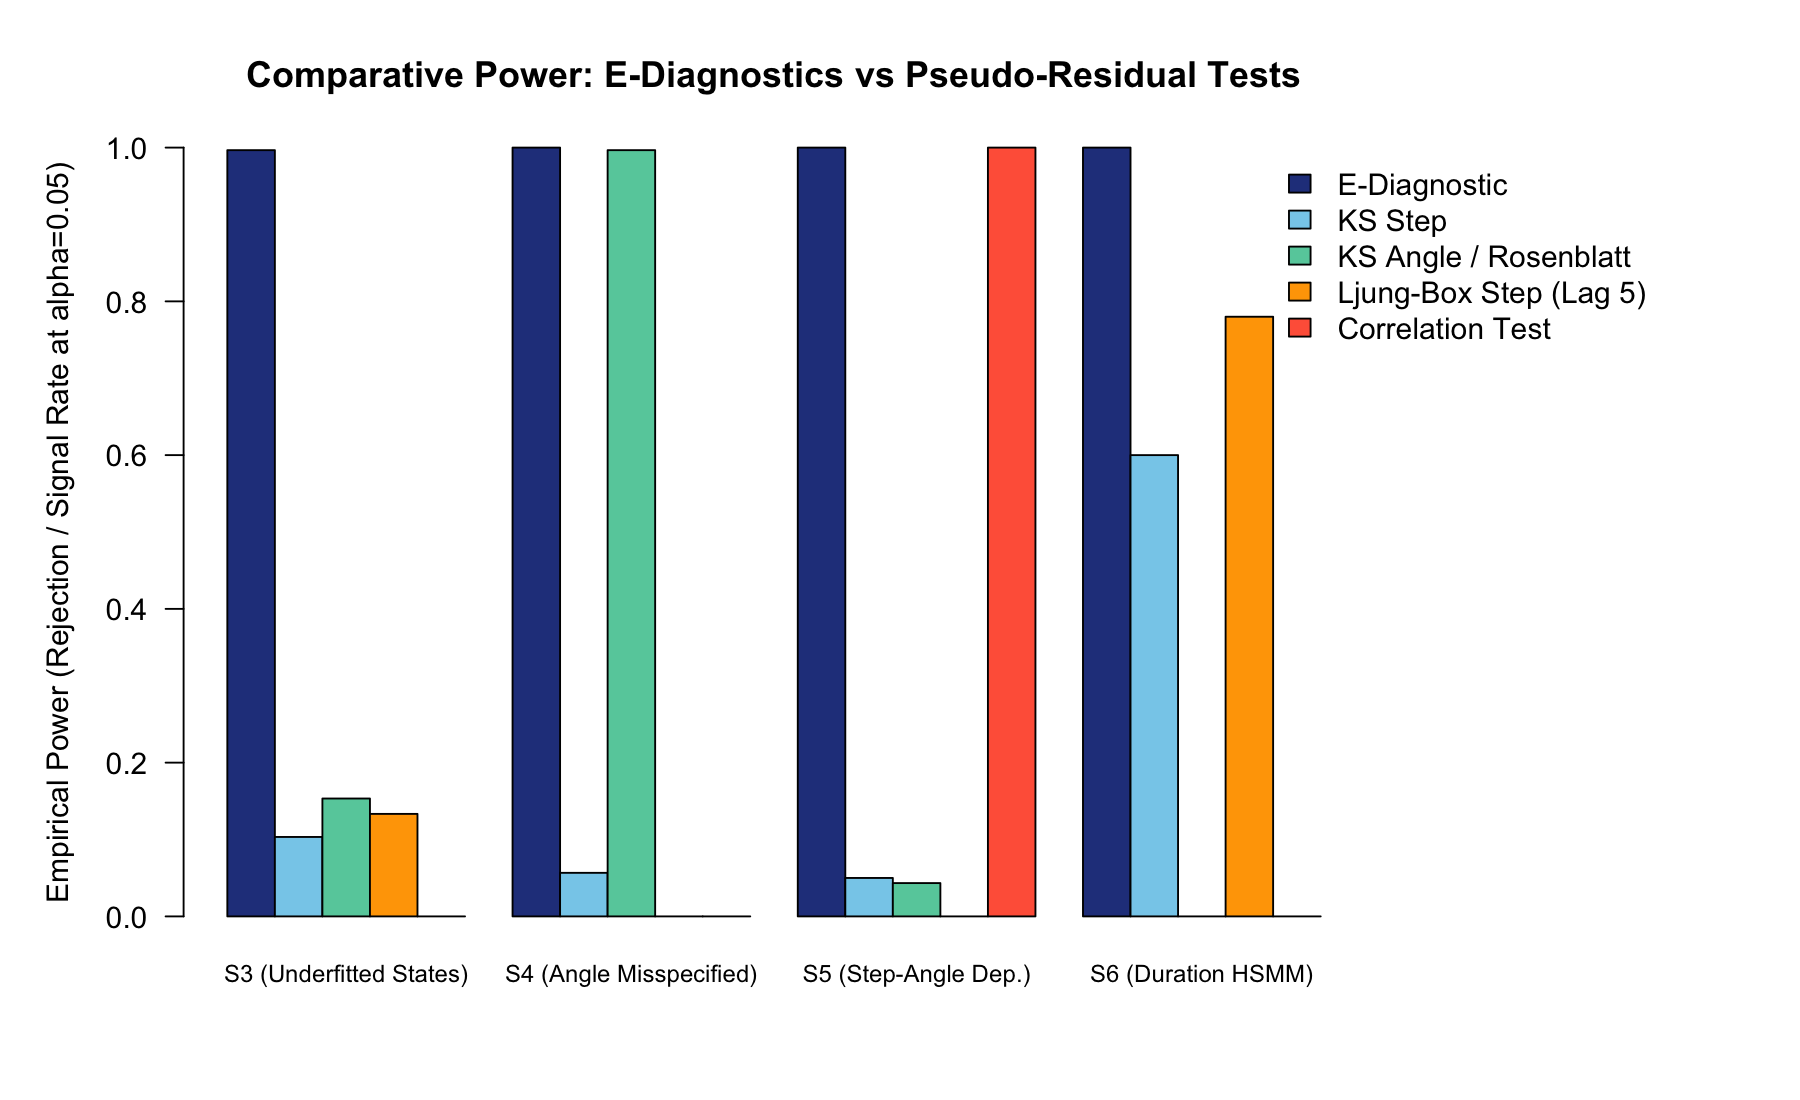
\includegraphics[width=0.92\linewidth]{comparative_power_residuals.png}
\caption{Threshold-crossing and retrospective rejection rates in scenarios S3--S6. All scenarios use 300 replicates; $T=300$ for S3--S5 and $T=500$ for S6.}
\label{fig:comparative_power_residuals}
\end{figure}

The comparison highlights how targeted e-diagnostics behave in these controlled scenarios:
\begin{enumerate}
\item Underfitted states (S3). The e-diagnostic detects the missing third state in 99.7\% of the replicates. The marginal Kolmogorov--Smirnov tests on steps and angles reject in 10.3\% and 15.3\% of the replicates, respectively, and the Ljung--Box autocorrelation test rejects in 13.3\%.
\item Angular misspecification (S4). Both the angular e-diagnostic and the marginal Kolmogorov--Smirnov test on turning angles have near-perfect rejection rates in this scenario (100\% and 99.7\%, respectively).
\item Step-angle joint dependence (S5). The copula e-diagnostic detects the residual dependence in 100\% of the replicates. The marginal Kolmogorov--Smirnov tests reject in 5.0\% and 4.3\% of the replicates because they target univariate deviations. The targeted correlation test on the joint normal residuals also rejects in 100\% of the replicates, but it remains a retrospective terminal test rather than an anytime-valid monitoring process.
\item Non-geometric state durations (S6). The blockwise duration e-diagnostic rejects in 100\% of the HSMM-like alternatives, whereas the step-length Kolmogorov--Smirnov test and Ljung--Box test reject in 60.0\% and 78.0\% of the replicates, respectively.
\end{enumerate}
These results show that, in the controlled alternatives considered here, e-diagnostics can be sensitive to structured misspecifications that are only weakly visible to marginal residual checks. They do not imply universal dominance over classical tests. The diagnostic alternatives in S3--S6 are targeted to the data-generating failures, and the classical tests reported here are retrospective tests whose p-values are not adjusted across tests, scenarios or sequential monitoring times.

\section{Elk movement application}
\label{sec:application}

As a real-data application, we used the elk movement data distributed as \texttt{elk\_data} in the R package \texttt{moveHMM} \citep{michelot_2016_movehmm}. The data are associated with the elk movement study of \citet{morales_2004_relocation}. The dataset contains four individuals and 735 locations with projected coordinates and distance to water. We used \texttt{moveHMM::prepData} to compute step lengths and turning angles. We implemented a Leave-One-Animal-Out (LOAO) cross-validation protocol: for each of the four individuals in turn, we held it out for validation and trained the candidate models on the remaining three individuals. Figure \ref{fig:elk_trajectory_split} displays the trajectories of the four individuals.

\begin{figure}[t]
\centering
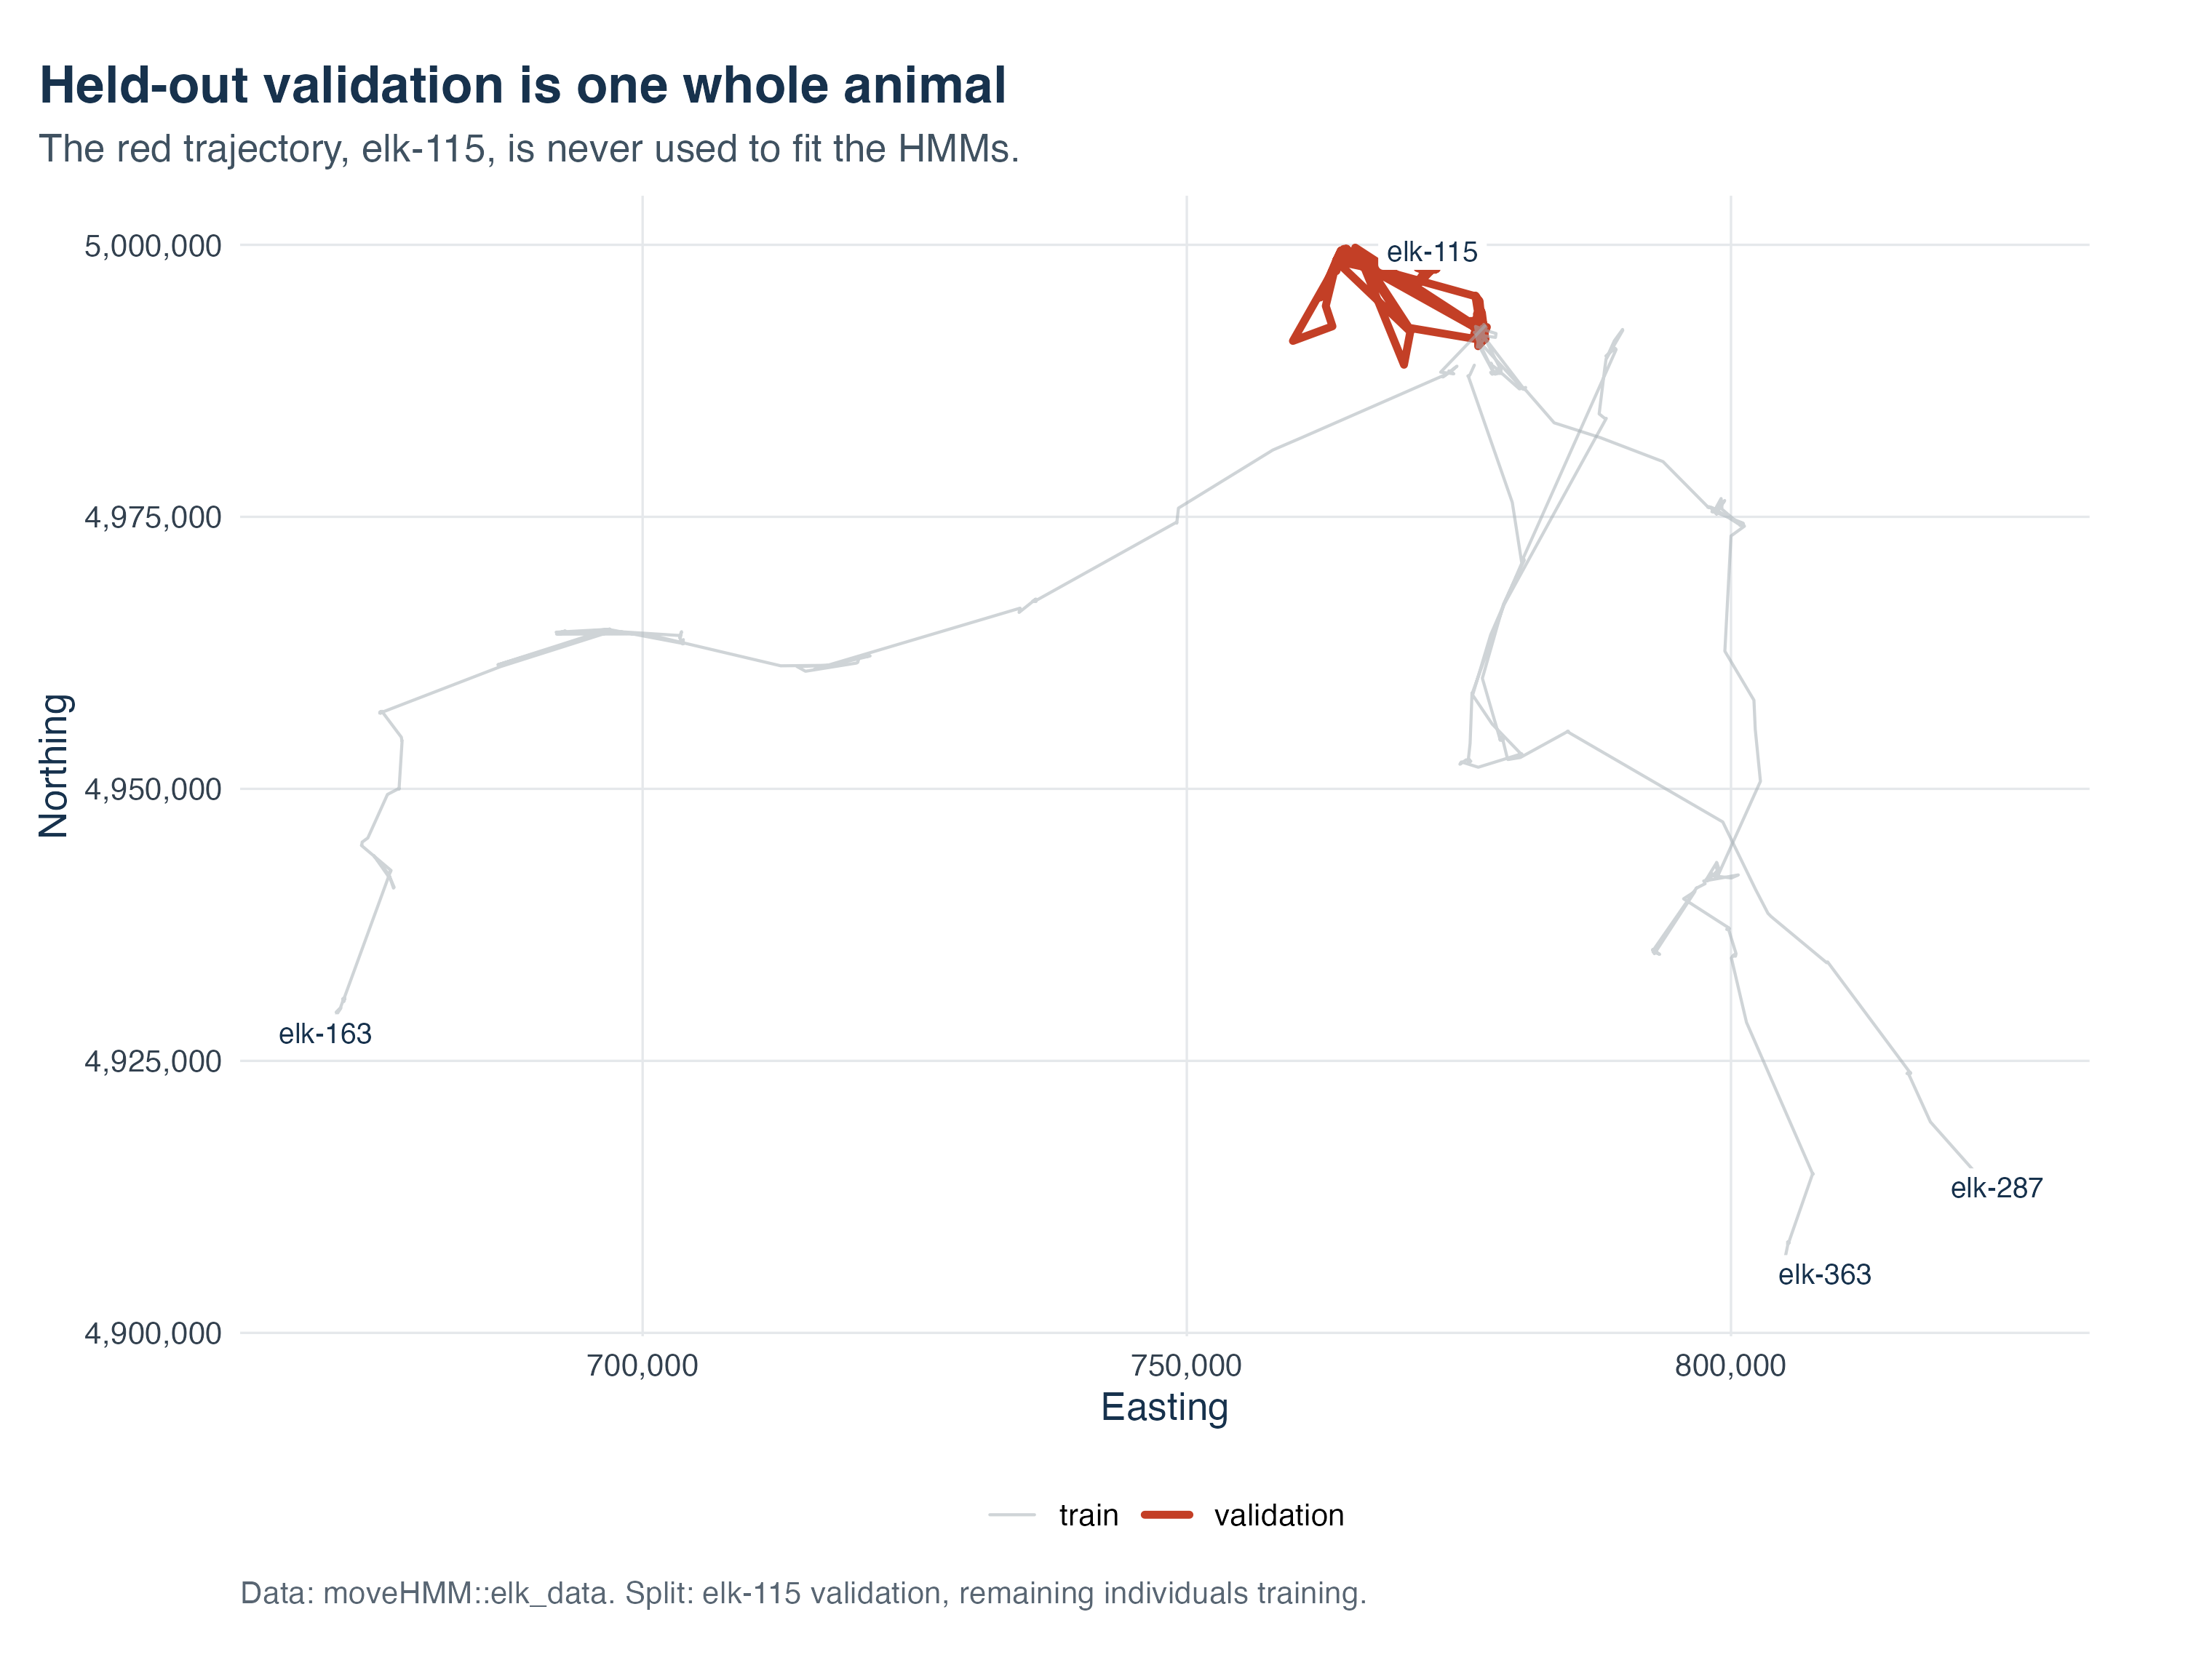
\includegraphics[width=\linewidth]{elk_trajectory_split.png}
\caption{Trajectories of the four elk individuals. Under the Leave-One-Animal-Out (LOAO) protocol, each trajectory is used for validation in turn.}
\label{fig:elk_trajectory_split}
\end{figure}

For each of the four folds, we fitted HMMs with $K=2,3,4$ states on the training individuals only, using Gamma step lengths and von Mises turning angles with no transition covariates. To reduce sensitivity to local optima, models were fitted using \texttt{moveHMM::fitHMM} from five deterministic initialization profiles based on the empirical step-length distribution and alternative angular-concentration patterns. The state distribution at the first observation was fixed to the stationary distribution. Label switching between cross-validation folds was resolved by ordering the states by their mean step lengths before prediction. The fixed mixture diagnostic allocated equal weight ($1/2$) to the $K=4$ density and the diffuse-angle density. Missing first steps or turning angles due to missing coordinates were dropped by \texttt{prepData}, and the filter was explicitly restarted for each individual to ensure valid prediction. The diffuse-angle diagnostic retains the fitted state weights and step length distributions, modifying only the turning angle density to a more diffuse von Mises distribution. All diagnostic choices were fixed before observing the validation trajectories. Figure \ref{fig:elk_model_selection} and Table \ref{tab:elk_model_selection} report the model-selection metrics. BIC selects $K=3$ as the null model for three folds (\texttt{elk-115}, \texttt{elk-287}, and \texttt{elk-363}) and $K=4$ for fold \texttt{elk-163}. To maintain consistency and allow population-level cross-fitted pooling, we fix the null generator to $K=3$ states and the diagnostic alternative to $K=4$ states across all validation individuals. Crucially, this decision rule (fixing the null to the majority model selected by BIC across training folds) was pre-specified before validation evidence was computed, ensuring that the model choice remains a predictable function of the training information $\calH$.

\begin{figure}[t]
\centering
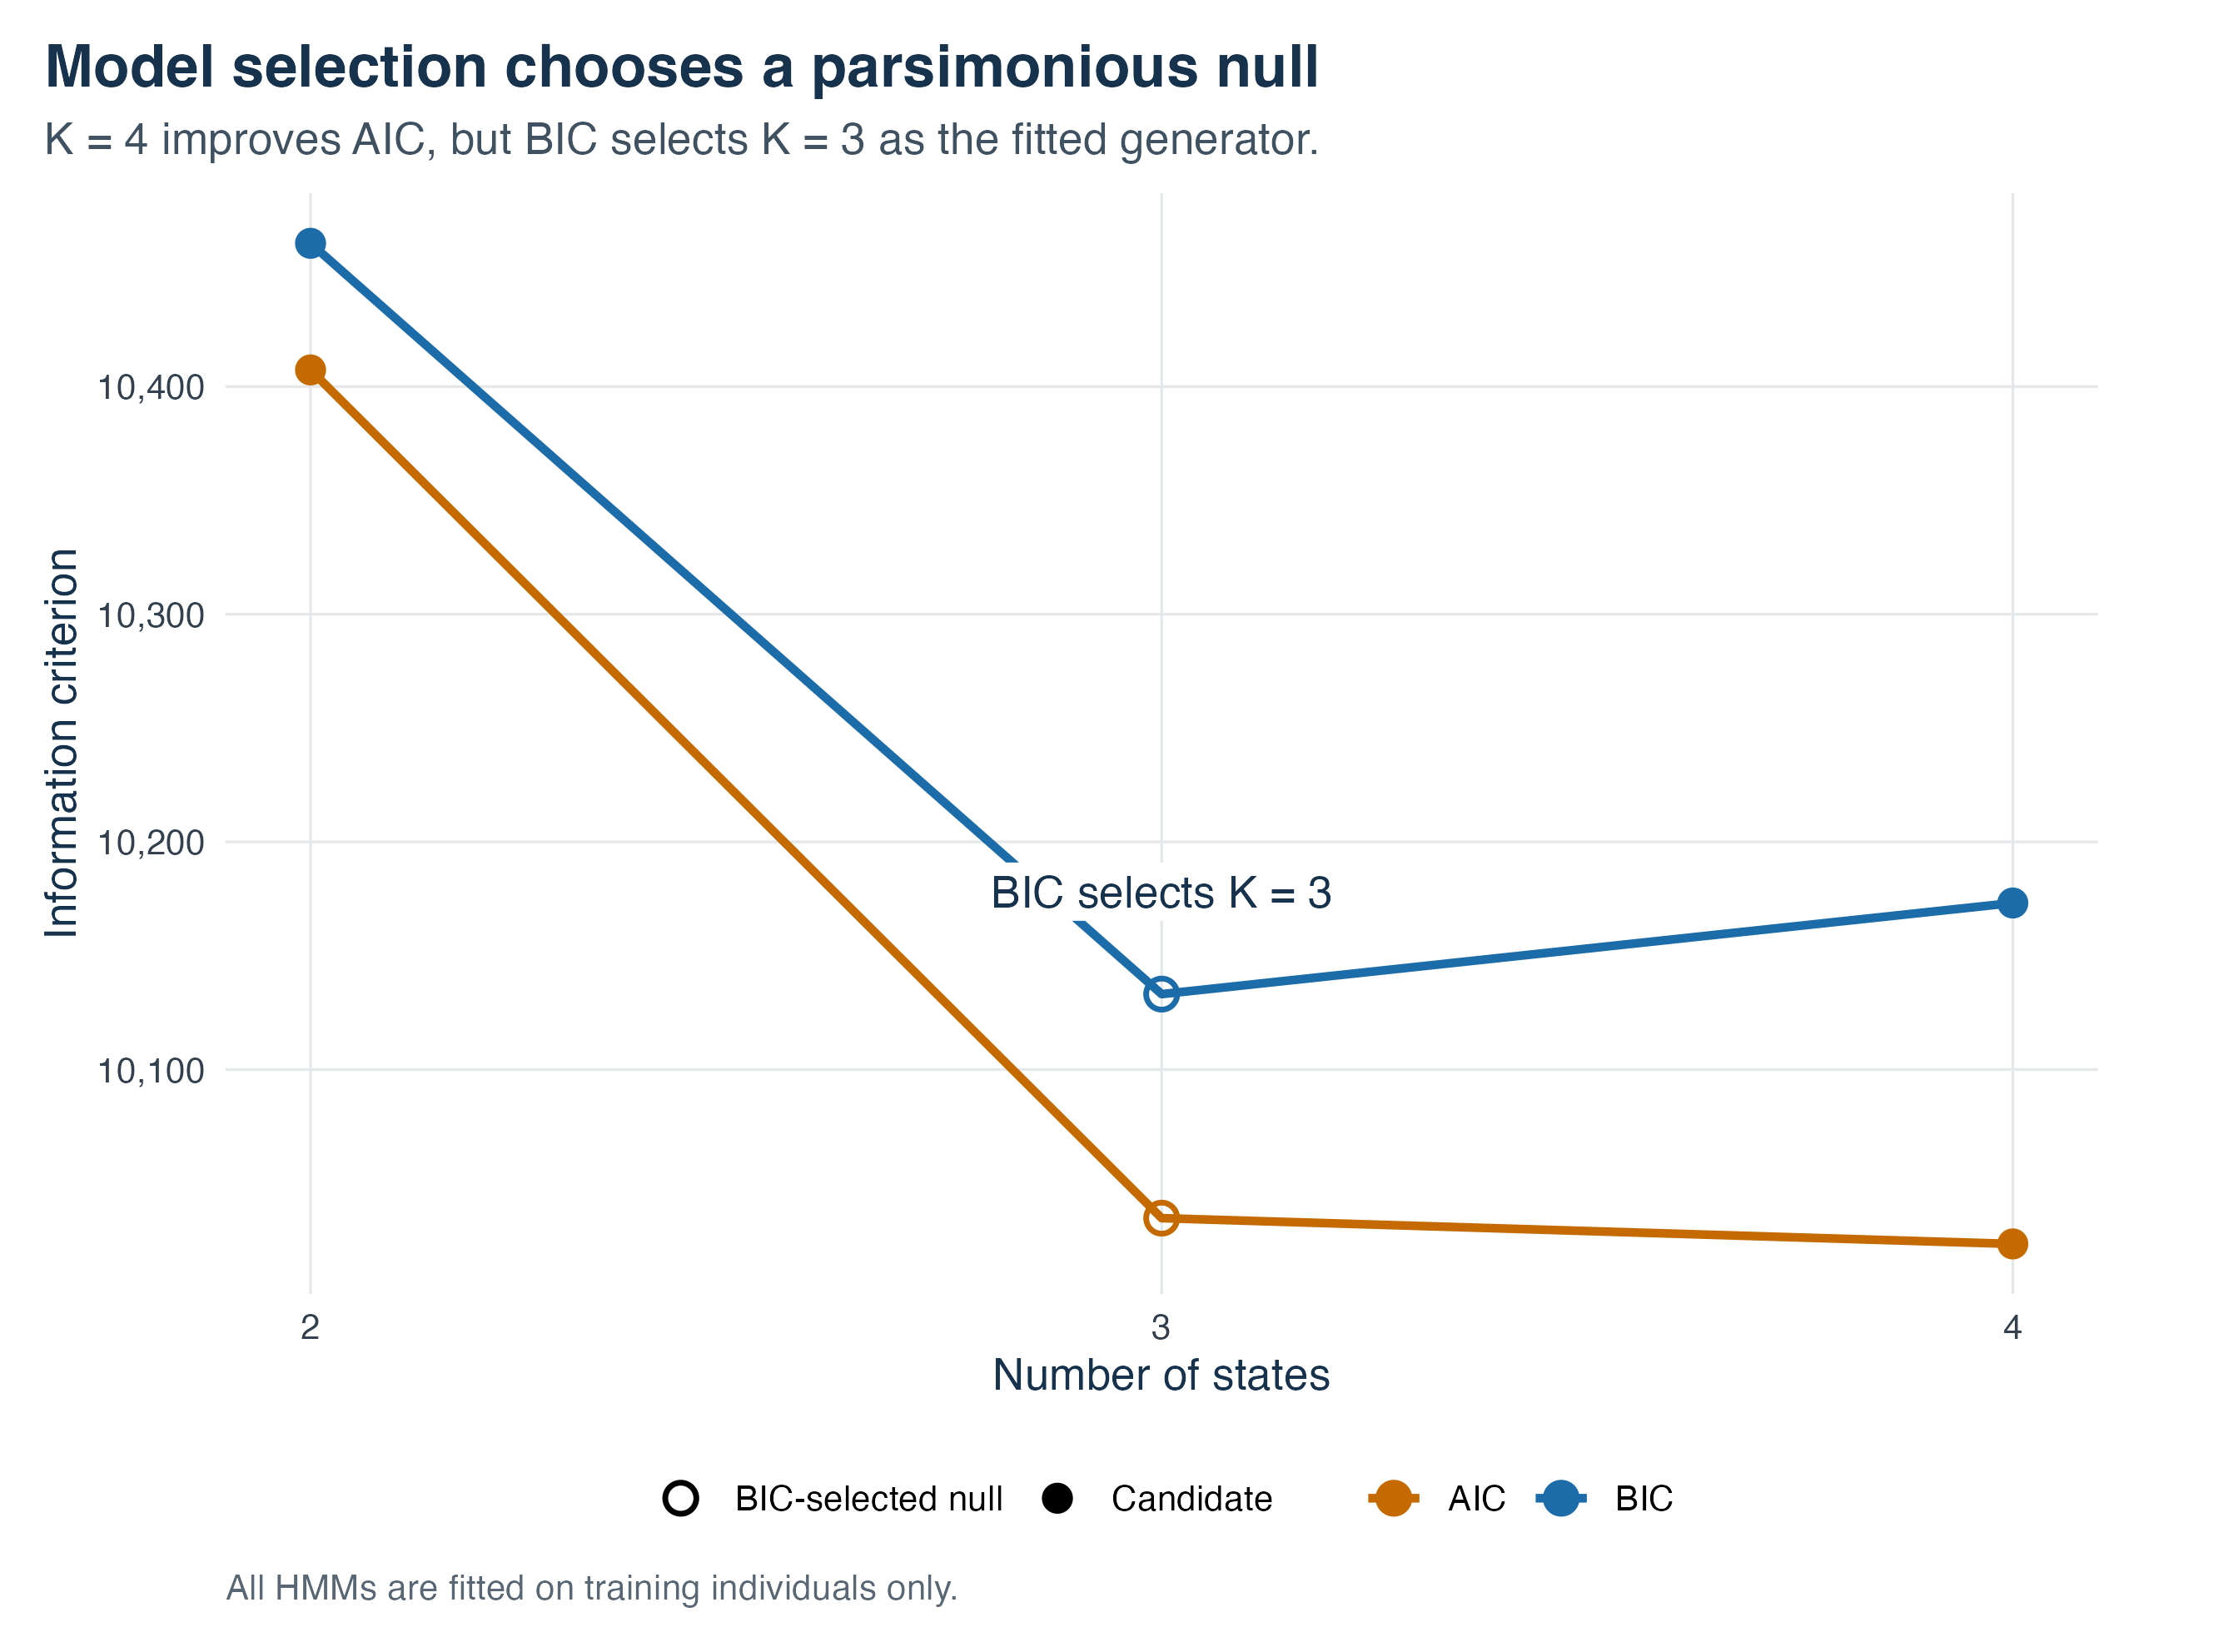
\includegraphics[width=0.92\linewidth]{elk_model_selection.png}
\caption{AIC and BIC for the fitted HMMs across the four training folds. BIC selects $K=3$ for three folds and $K=4$ for one fold.}
\label{fig:elk_model_selection}
\end{figure}

\begin{table}[t]
\centering
\footnotesize
\begin{tabular}{lccccr}
\toprule
Fold (Validation Indiv.) & States ($K$) & Negative Log-Likelihood & Parameters & AIC & BIC \\
\midrule
\textbf{elk-115} & 2 & 5190.649 & 13 & 10407.298 & 10462.919 \\
(Training $n = 533$) & 3 & 4994.368 & 23 & 10034.736 & 10133.142$^\star$ \\
                     & 4 & 4976.707 & 35 & 10023.414 & 10173.162 \\
\addlinespace
\textbf{elk-163} & 2 & 5442.706 & 13 & 10911.412 & 10967.860 \\
(Training $n = 568$) & 3 & 5378.781 & 23 & 10803.562 & 10903.430 \\
                     & 4 & 5335.920 & 35 & 10741.841 & 10893.815$^\star$ \\
\addlinespace
\textbf{elk-287} & 2 & 5481.246 & 13 & 10988.493 & 11044.826 \\
(Training $n = 563$) & 3 & 5332.742 & 23 & 10711.484 & 10811.149$^\star$ \\
                     & 4 & 5297.755 & 35 & 10665.510 & 10817.175 \\
\addlinespace
\textbf{elk-363} & 2 & 4999.619 & 11 & 10021.237 & 10067.837 \\
(Training $n = 511$) & 3 & 4830.232 & 20 & 9700.463 & 9785.190$^\star$ \\
                     & 4 & 4813.181 & 31 & 9688.363 & 9819.690 \\
\bottomrule
\end{tabular}
\caption{Model selection metrics for fitted HMMs across Leave-One-Animal-Out training sets. The $^\star$ symbol denotes the model selected by BIC for each fold.}
\label{tab:elk_model_selection}
\end{table}

We then evaluated four diagnostics on each validation individual: a full-density $K+1$ diagnostic comparing the $K=3$ null HMM with the $K=4$ alternative HMM, a diffuse-angle diagnostic obtained by halving the fitted angular concentrations under the null, a fixed mixture of these two diagnostic densities (allocating equal weight to each), and a state-localized version of the $K+1$ diagnostic using the filtered predictive probability of the long-step state. Figure \ref{fig:elk_eprocess_paths} shows the resulting cumulative paths for the four individuals, and Table \ref{tab:elk_diagnostics} summarizes their crossings, maxima, and final values, alongside the population-average cross-fitted e-values (Proposition~\ref{prop:crossfit_average}).

\begin{figure}[t]
\centering
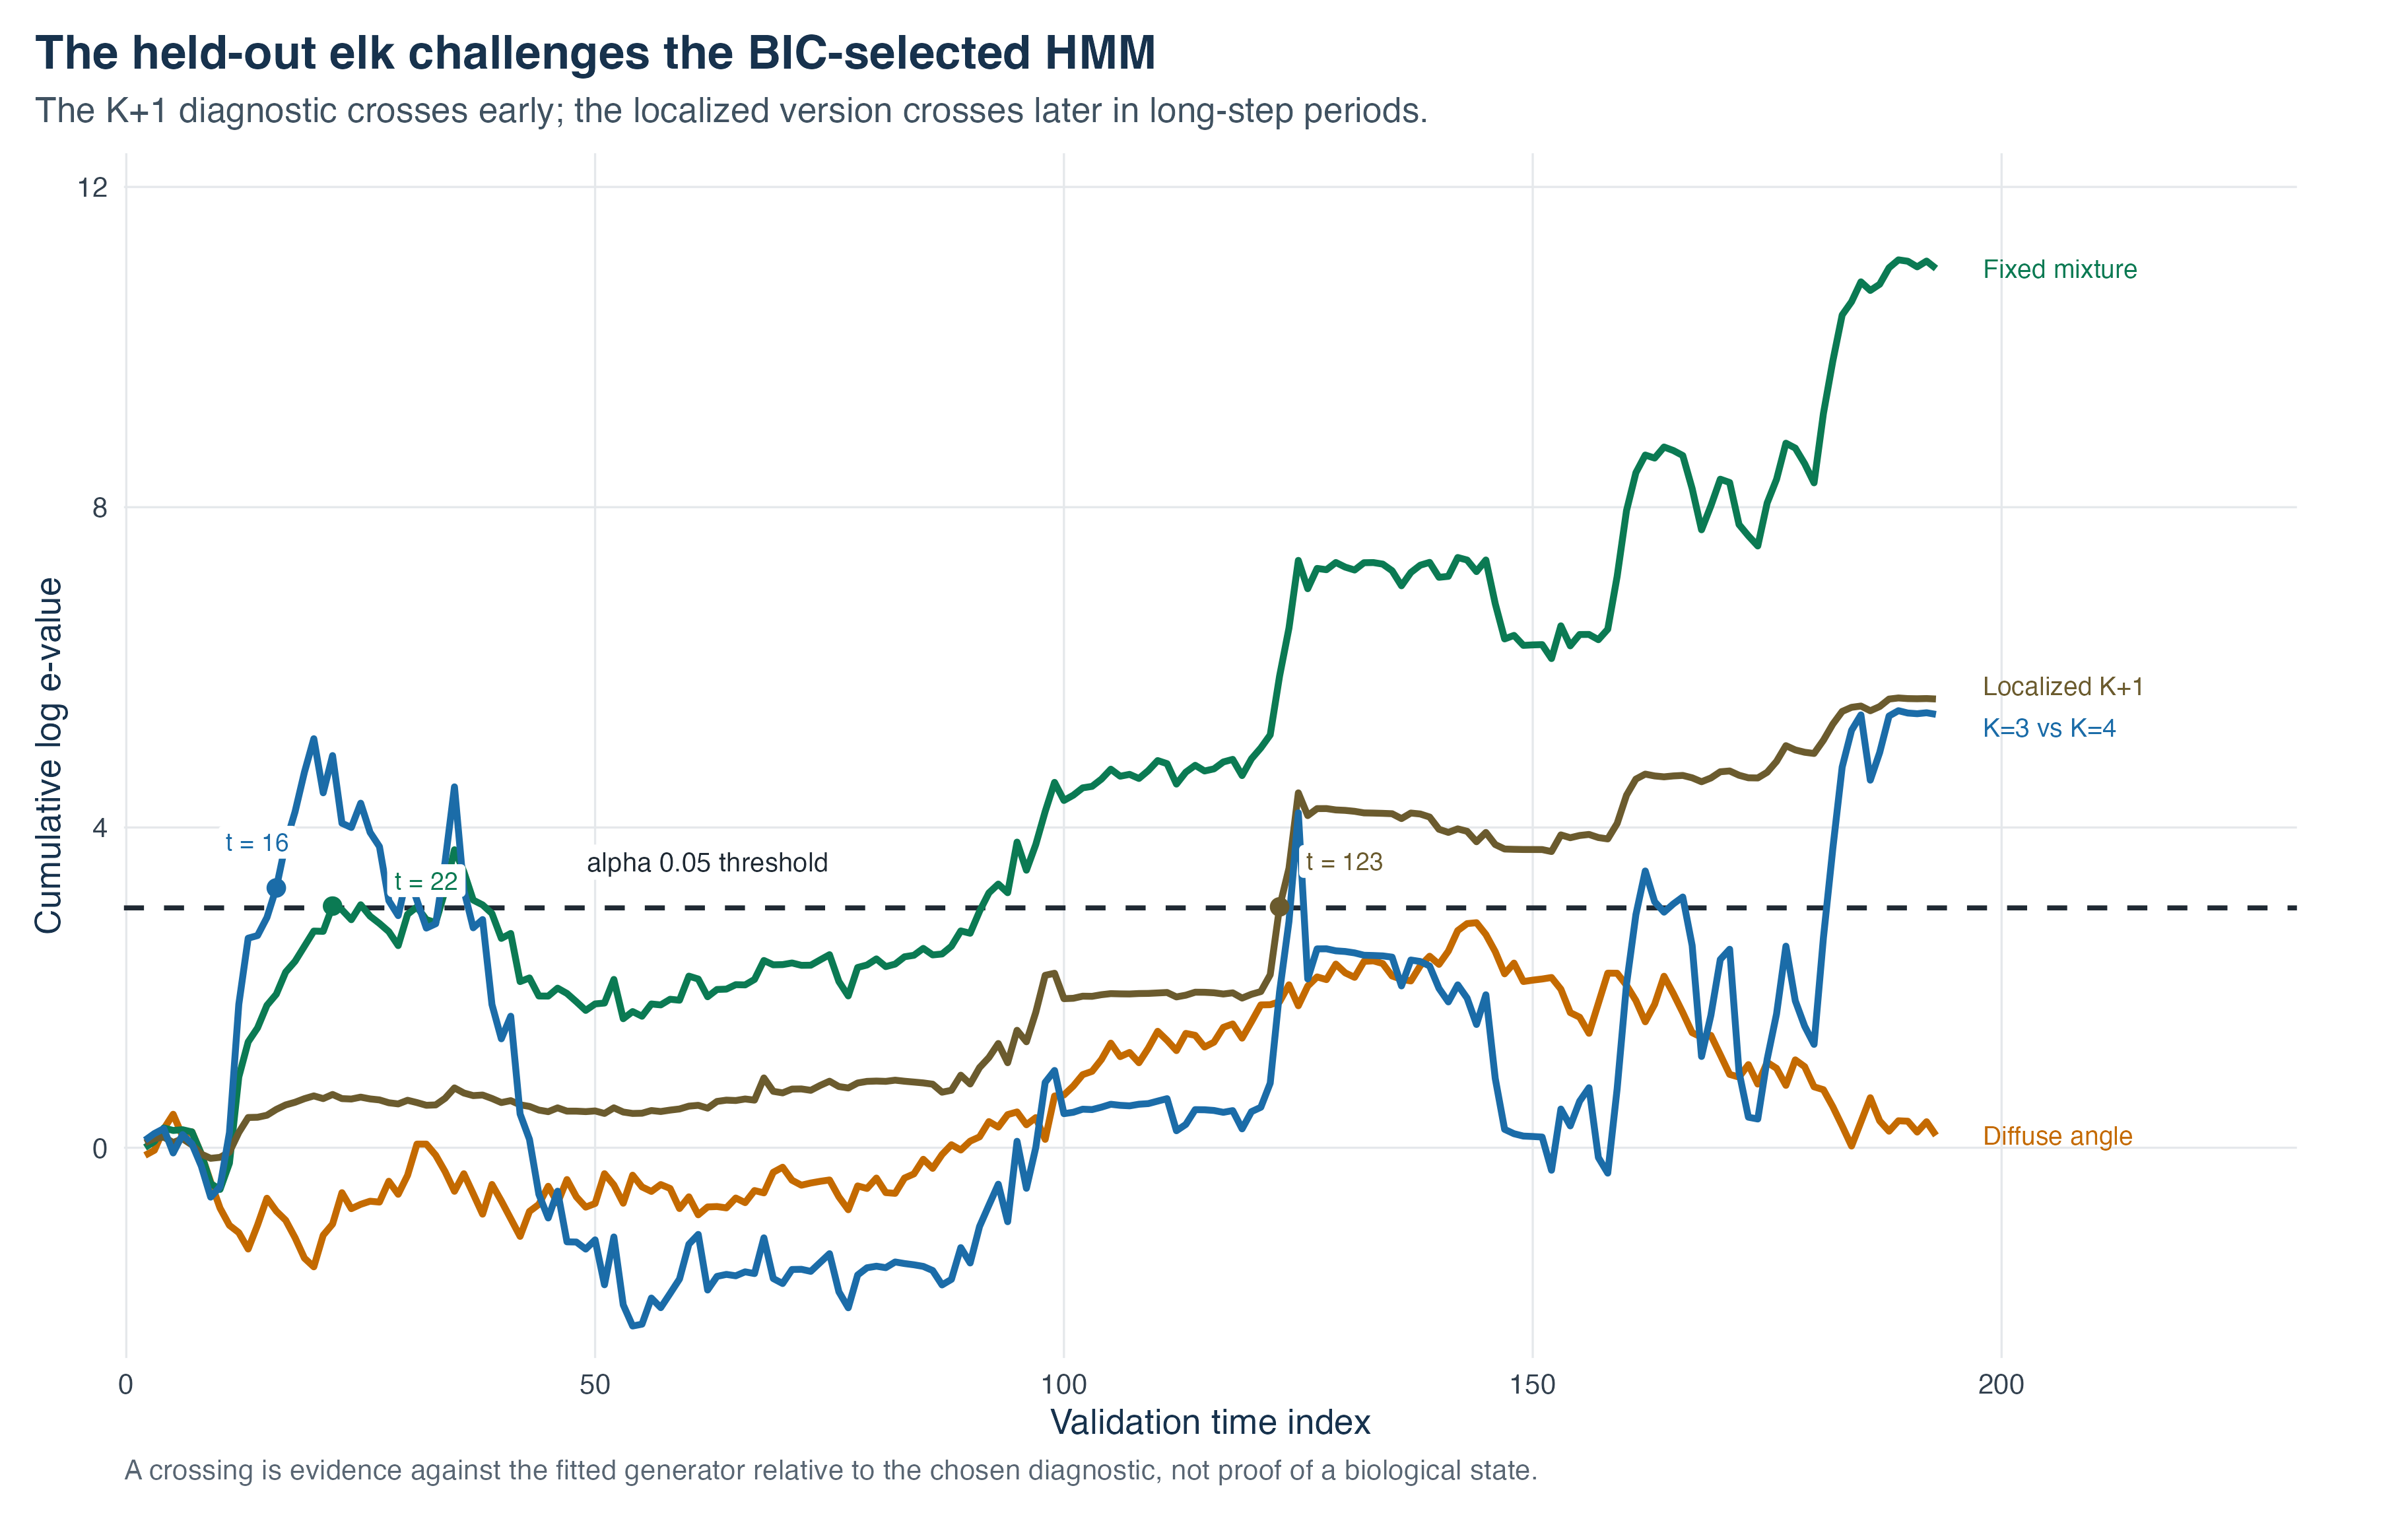
\includegraphics[width=\linewidth]{elk_eprocess_paths.png}
\caption{Cumulative log e-processes for the four validation elk individuals across the four diagnostics. The dashed horizontal line is the $\alpha=0.05$ threshold, $\log(20) = 2.996$.}
\label{fig:elk_eprocess_paths}
\end{figure}

\begin{table}[t]
\centering
\footnotesize
\begin{tabular}{lcccc}
\toprule
Validation Individual / Diagnostic & Crossed? & Crossing Time & Max $\log e$ & Final $\log e$ \\
\midrule
\textbf{elk-115} ($n = 192$) & & & & \\
\quad $K=3$ vs $K=4$ & Yes & 16 & 5.459 & 5.413 \\
\quad Diffuse angle & No & NA & 2.811 & 0.154 \\
\quad Fixed mixture & Yes & 22 & 11.089 & 10.981 \\
\quad Localized $K+1$ & Yes & 123 & 5.618 & 5.605 \\
\addlinespace
\textbf{elk-163} ($n = 157$) & & & & \\
\quad $K=3$ vs $K=4$ & No & NA & 0.610 & -12.216 \\
\quad Diffuse angle & Yes & 109 & 3.585 & 2.663 \\
\quad Fixed mixture & No & NA & 1.556 & -1.244 \\
\quad Localized $K+1$ & No & NA & 0.165 & -1.725 \\
\addlinespace
\textbf{elk-287} ($n = 162$) & & & & \\
\quad $K=3$ vs $K=4$ & No & NA & 1.854 & 1.056 \\
\quad Diffuse angle & No & NA & 2.220 & 1.801 \\
\quad Fixed mixture & No & NA & 2.836 & 2.592 \\
\quad Localized $K+1$ & No & NA & 0.619 & 0.513 \\
\addlinespace
\textbf{elk-363} ($n = 214$) & & & & \\
\quad $K=3$ vs $K=4$ & Yes & 118 & 13.627 & 7.246 \\
\quad Diffuse angle & No & NA & 1.337 & -0.761 \\
\quad Fixed mixture & Yes & 116 & 9.973 & 9.174 \\
\quad Localized $K+1$ & Yes & 212 & 5.095 & 4.734 \\
\midrule
\textbf{Population Average} ($N = 4, n_{tot} = 725$) & & & & \\
\quad $K=3$ vs $K=4$ & Yes & NA & 6.009 & 6.009 \\
\quad Diffuse angle & No & NA & 1.706 & 1.706 \\
\quad Fixed mixture & Yes & NA & 9.747 & 9.747 \\
\quad Localized $K+1$ & Yes & NA & 4.573 & 4.573 \\
\bottomrule
\end{tabular}
\caption{Leave-One-Animal-Out predictive e-diagnostics for the four elk individuals and the population-average cross-fitted e-values. The threshold for $\alpha=0.05$ is $\log(20) = 2.996$. For the population average, the final log e-value represents $\log E^{\text{cf}}$ and the max log e-value is identical to the final value by definition.}
\label{tab:elk_diagnostics}
\end{table}

The diagnostics show substantial variation across individuals. For \texttt{elk-115} and \texttt{elk-363}, the $K+1$ state diagnostic and the fixed mixture cross the standard threshold $1/\alpha = 20$ ($\log(20) = 2.996$), suggesting that the three-state null HMM is inadequate for these trajectories. The state-localized diagnostic also crosses for these two individuals, supporting the interpretation that the predictive discrepancy is concentrated during periods assigned high probability of the long-step state. For \texttt{elk-163}, the diffuse-angle diagnostic crosses the threshold, suggesting that the diffuse-angle diagnostic predicts this trajectory better than the fitted angular component for this animal, while the diagnostic for the number of states does not cross. For \texttt{elk-287}, none of the individual diagnostics cross the threshold.

Importantly, evaluating multiple diagnostics post-hoc on the same individuals requires multiple-testing discipline if one wishes to make joint confirmatory statements rather than exploratory reporting. With $J = 4$ parallel diagnostics, a Bonferroni-style union bound adjustment can be applied by setting the significance level for each diagnostic to $\alpha/J = 0.0125$. This corresponds to an anytime-valid threshold of $J/\alpha = 80$, or $\log(80) \approx 4.382$ in the log scale. Under this conservative adjusted threshold, the number-of-states diagnostic and the fixed mixture still cross for \texttt{elk-115} and \texttt{elk-363}, and the state-localized diagnostic still crosses for \texttt{elk-115}, while the diffuse-angle diagnostic for \texttt{elk-163} no longer crosses (maximum $\log E = 3.585$).

Importantly, Proposition~\ref{prop:crossfit_average} allows us to pool evidence across individuals using the population-average cross-fitted e-value, $E^{\text{cf}} = \frac{1}{N} \sum_{i=1}^N E^{(i)}$. Because every individual is simultaneously both a validation unit and part of the training set for other folds, presenting LOAO as an exact global test requires caution, as the overlapping training sets make the "fixed fitted generator" interpretation less clean. More rigorously, conditional on the training set for fold $i$, $E^{(i)}$ is valid for the hypothetical validation law generated by the fold-specific fitted model. The population-average $E^{\text{cf}}$ is valid if all fold-specific validation laws are embedded in a common joint null under which each $E^{(i)}$ has expectation at most one. Under this interpretation, $E^{\text{cf}}$ remains a valid population-level cross-predictive diagnostic. However, because $E^{\text{cf}}$ is an arithmetic average, it can be dominated by one or two large individual e-values and is not a measure of typical individual fit. For example, in Table \ref{tab:elk_diagnostics}, the population average for $K+1$ states ($\log E^{\text{cf}} = 6.009$) is heavily influenced by the large positive values for \texttt{elk-115} and \texttt{elk-363}, despite a negative log e-value for \texttt{elk-163}. Thus, a complementary display of individual-level evidence is essential, and population-level claims should be interpreted cautiously.

As shown in Table \ref{tab:elk_diagnostics} and Figure \ref{fig:elk_diagnostic_summary}, the population-average log e-value exceeds the terminal e-value threshold for the diagnostic for the number of states ($\log E^{\text{cf}} = 6.009$), the fixed mixture ($\log E^{\text{cf}} = 9.747$), and the localized diagnostic ($\log E^{\text{cf}} = 4.573$). Only the diffuse-angle diagnostic does not exceed the terminal threshold at the population level ($\log E^{\text{cf}} = 1.706$). In this illustrative dataset, the LOAO diagnostics suggest that the three-state fitted generator is inadequate for some held-out individuals, with population-average evidence concentrated in the number-of-states and long-step-localized diagnostics. Figure \ref{fig:elk_state_localization} shows the predictable state weights and localized cumulative e-process for \texttt{elk-115}.

\begin{figure}[t]
\centering
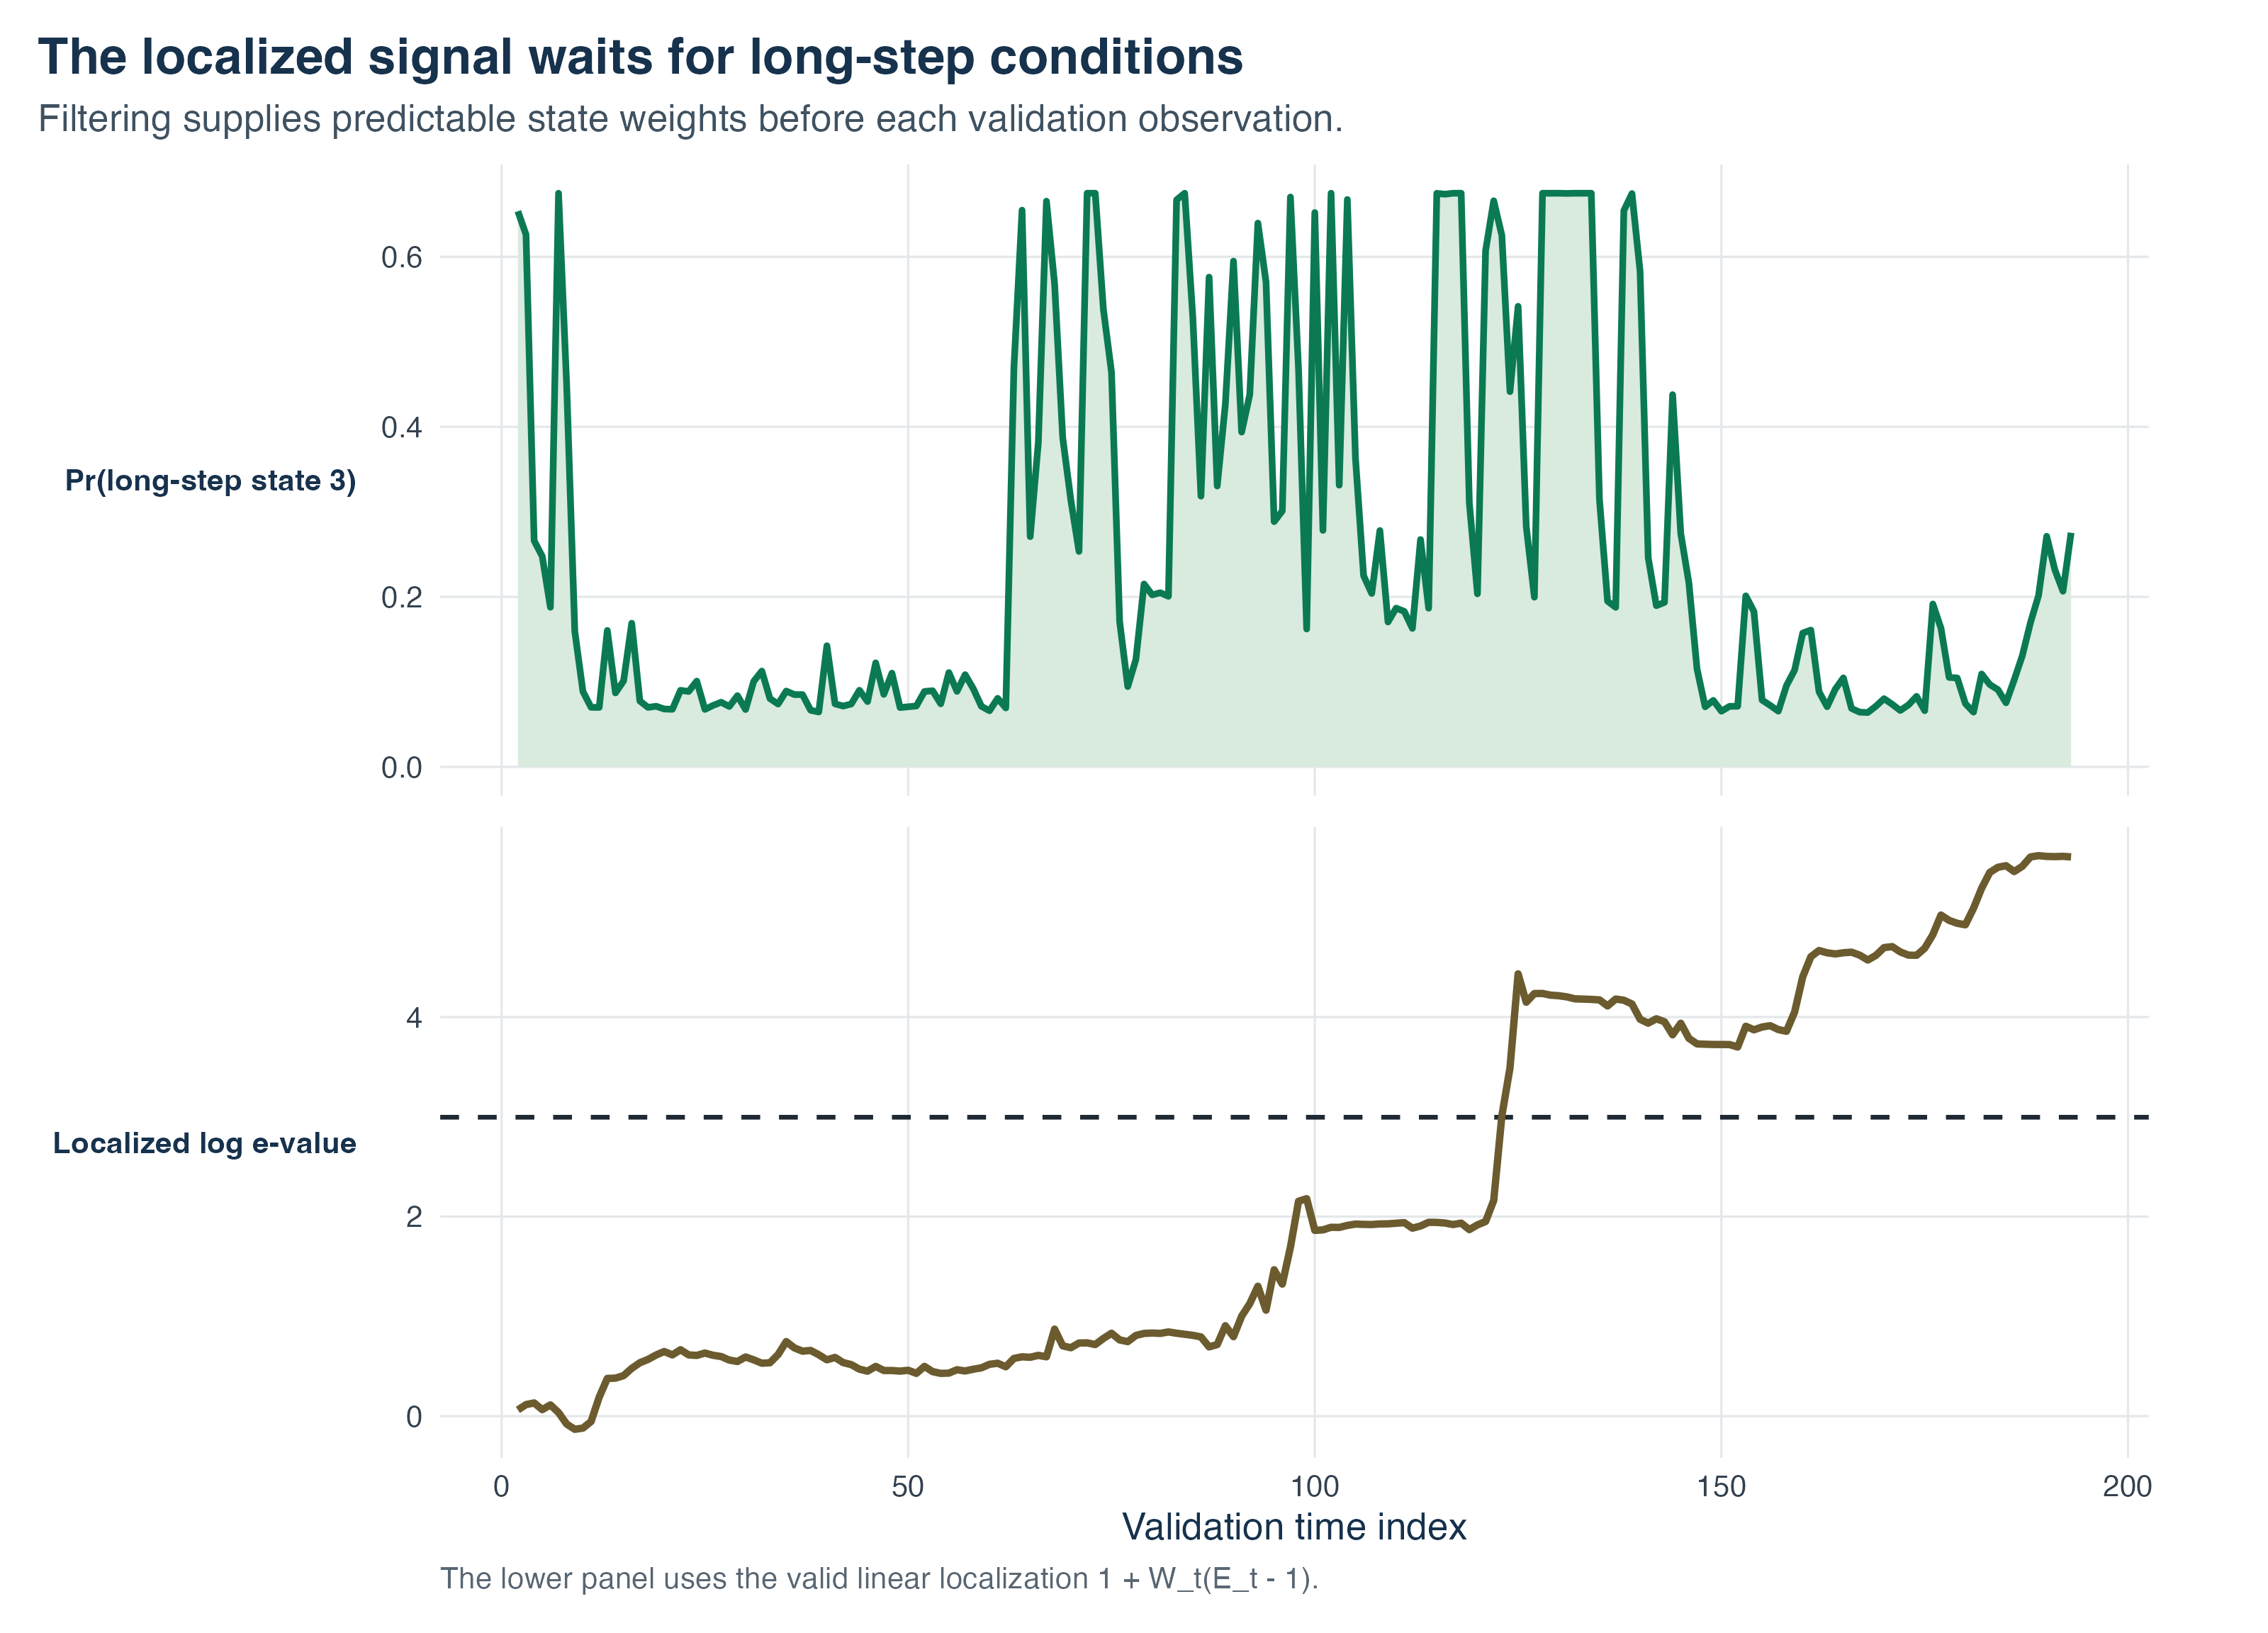
\includegraphics[width=\linewidth]{elk_state_localization.png}
\caption{Predictable state-localized diagnostic for validation individual \texttt{elk-115}. The upper panel shows the filtered predictive probability assigned to the long-step state before each validation observation. The lower panel shows the corresponding localized cumulative log e-process.}
\label{fig:elk_state_localization}
\end{figure}

\begin{figure}[t]
\centering
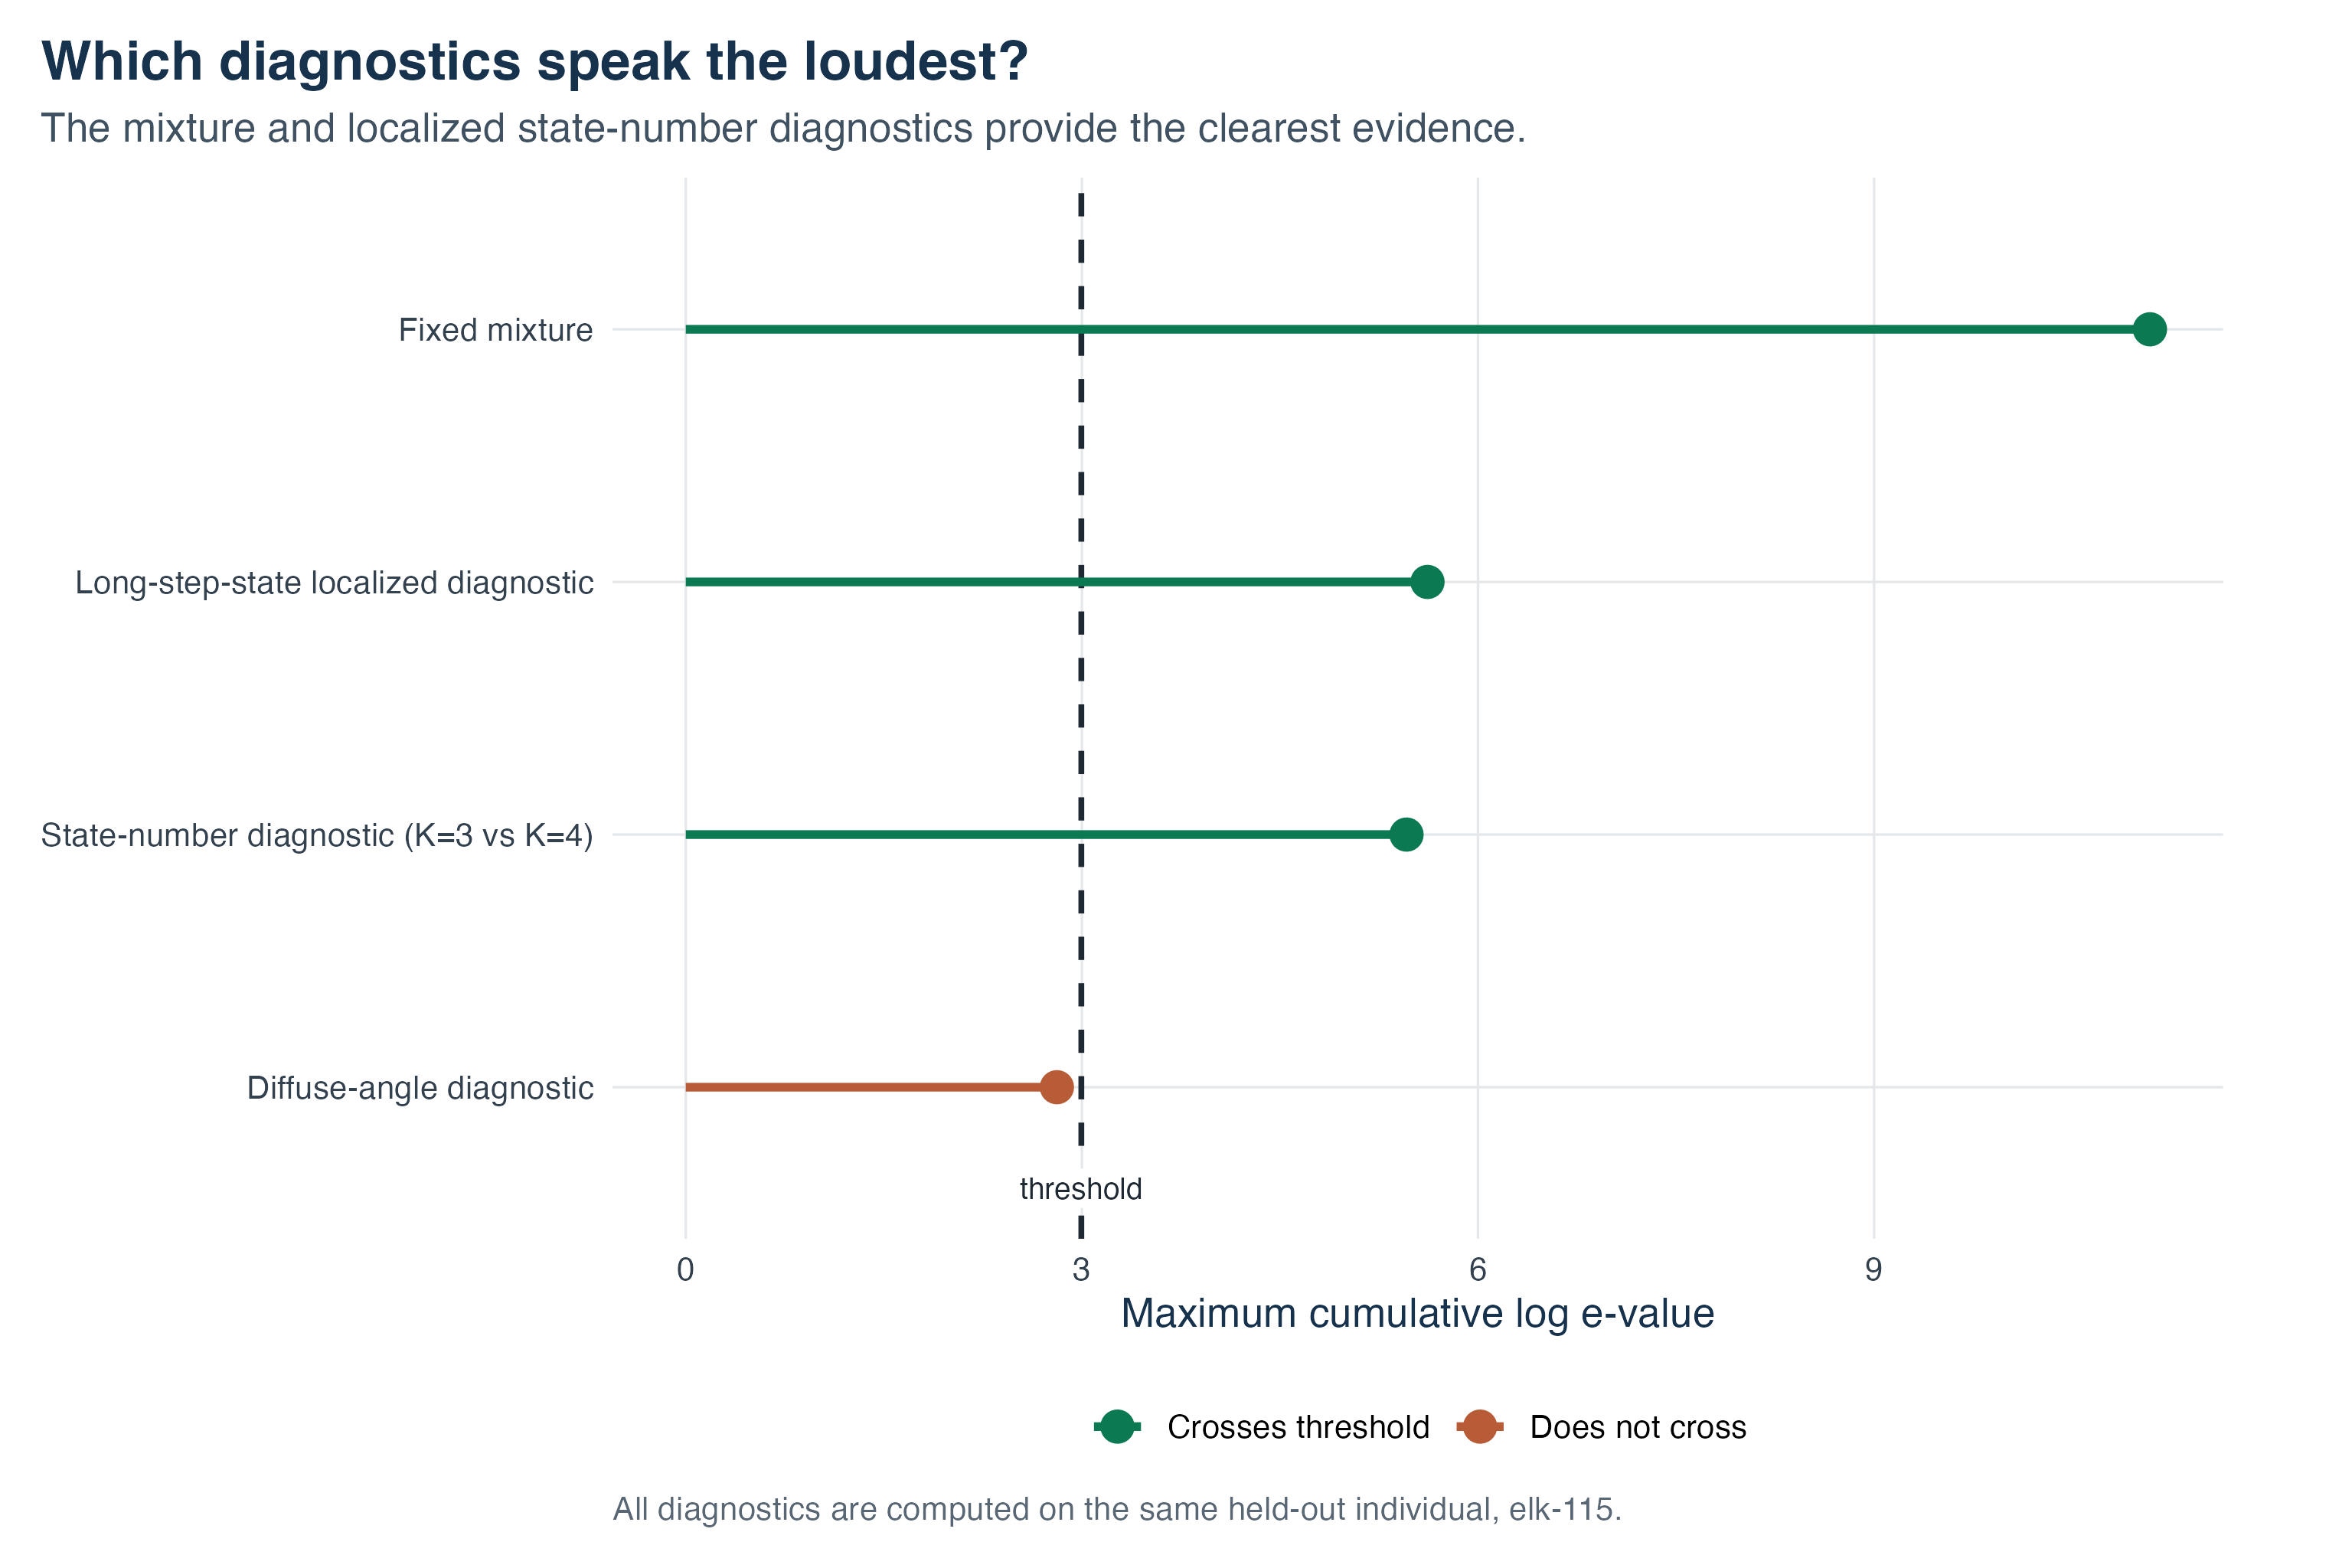
\includegraphics[width=0.9\linewidth]{elk_diagnostic_summary.png}
\caption{Summary of final log e-values across validation individuals (circles) and the population-average cross-fitted e-value (diamond marker). The dashed line represents the $\alpha=0.05$ threshold, $\log(20) = 2.996$.}
\label{fig:elk_diagnostic_summary}
\end{figure}

This application illustrates the Leave-One-Animal-Out cross-fitted workflow: train the HMM on a subset of individuals, specify diagnostic alternatives, evaluate the e-processes on held-out animals, and compute population-level cross-fitted e-values to pool evidence. The results illustrate how predictive e-diagnostics can reveal individual-specific lack of predictive fit and can be combined into a population-level terminal e-value.

\section{Discussion}
\label{sec:discussion}

This theoretical framework turns model checking for multi-state movement models into a sequence of explicit predictive bets. The null HMM is assessed as a sequential generator of held-out movement data. The latent states are integrated out through filtering. Diagnostic alternatives define targeted predictive competitors. The resulting cumulative ratios are e-processes under the fixed train/validation null, giving anytime-valid thresholds for sequential model criticism.

The framework adds several elements that are specific to movement HMMs. First, it prevents a common conceptual error: e-validity is based on the observable predictive density, not on a density conditional on decoded states. Second, it provides a way to localize model failure using predictable weights, including habitat indicators and filtered state probabilities. Third, it supports diagnostics tailored to movement structure: turning-angle misspecification, residual circular-linear dependence, non-geometric dwell times and long-horizon spatial behaviour. Fourth, it clarifies how several diagnostics can be combined. Predictable switching and mixtures are valid; parallel products on the same validation observations are not valid by default.

The main limitation is the treatment of fitted parameters. The exact guarantee is cleanest when the fitted null and diagnostic alternatives are fixed before validation. This is a strength for a first methodological article because the null statement is transparent: conditional on training, does the fitted HMM generate the validation trajectory credibly? Same-sample exploratory workflows are still useful but require caution. The supplementary simulations therefore treat oracle-state parameter estimation, validation by individuals and composite-null envelopes as sensitivity analyses or extensions rather than as the main empirical evidence.

The sequential-workflow result also gives a formal language for exploratory data analysis of fitted movement models. An analyst can inspect one diagnostic signal, decide that a state-localized, time-localized or feature-level diagnostic is the next relevant question, and continue with a conditionally valid e-value if that next diagnostic is based on information not already used in an invalid way. This is not a license for unrecorded post-hoc selection on the same observations; rather, it separates controlled sequential exploration from descriptive follow-up.

The real-data example illustrates both the promise and the caution required in practice. Predictive e-diagnostics can reveal that a fitted generator performs poorly for a held-out animal, and localized versions help identify the part of the fitted behavioural structure associated with the signal. At the same time, ecological interpretation requires additional work: the diagnostic menu, train/validation split and model-selection rule should be pre-specified for confirmatory use, and the results should be replicated across datasets or validation splits before drawing definitive biological conclusions.

Several extensions are natural but outside the scope of this first HMM-focused article. These include predictive e-diagnostics for HMM step-selection or integrated step-selection formulations, diagnostics connected to visual inference workflows, and prediction-powered variants that use external predictive models as diagnostic competitors. The accompanying experimental R package, \texttt{evalueHMM}, provides an initial implementation of the HMM-focused diagnostics developed here; extensions beyond this scope would require their own statements of the validation filtration, predictable covariates and null target.


\section*{Code and Data Availability}
The elk data used in the application are publicly available in the supplementary materials of \cite{michelot_2016_movehmm} and via the \texttt{moveHMM} package. The repository is an installable R package and reproducible research compendium for \texttt{evalueHMM}; it contains package functions, R scripts, simulation parameters, random seeds, and a README to reproduce the tables and figures by rerunning the simulation and application scripts. While generated outputs are ignored by Git as noted in the supplement, the verifiable results and full scripts can be accessed at \url{https://github.com/AurelienNicosiaULaval/evalue-HMM}.

\begin{thebibliography}{99}

\bibitem[Dawid(1984)]{dawid_1984_prequential}
Dawid, A. P. (1984).
Statistical theory: the prequential approach.
\emph{Journal of the Royal Statistical Society. Series A}, 147(2), 278--292.
\url{https://doi.org/10.2307/2981683}

\bibitem[Gr{\"u}nwald et~al.(2024)]{grunwald_2024_safe_testing}
Gr{\"u}nwald, P., de Heide, R., and Koolen, W. M. (2024).
Safe testing.
\emph{Journal of the Royal Statistical Society: Series B}, 86(5), 1091--1128.
\url{https://doi.org/10.1093/jrsssb/qkae011}

\bibitem[Howard et~al.(2020)]{howard_2020_time_uniform}
Howard, S. R., Ramdas, A., McAuliffe, J., and Sekhon, J. (2020).
Time-uniform Chernoff bounds via nonnegative supermartingales.
\emph{Probability Surveys}, 17, 257--317.
\url{https://doi.org/10.1214/18-PS321}

\bibitem[Langrock et~al.(2012)]{langrock_2012_telemetry}
Langrock, R., King, R., Matthiopoulos, J., Thomas, L., Fortin, D., and Morales, J. M. (2012).
Flexible and practical modeling of animal telemetry data: hidden Markov models and extensions.
\emph{Ecology}, 93(11), 2336--2342.
\url{https://doi.org/10.1890/11-2241.1}

\bibitem[Langrock and Zucchini(2011)]{langrock_zucchini_2011_dwell}
Langrock, R. and Zucchini, W. (2011).
Hidden Markov models with arbitrary state dwell-time distributions.
\emph{Computational Statistics \& Data Analysis}, 55(1), 715--724.
\url{https://doi.org/10.1016/j.csda.2010.06.015}

\bibitem[McClintock and Michelot(2018)]{mcclintock_2018_momentuhmm}
McClintock, B. T. and Michelot, T. (2018).
\texttt{momentuHMM}: R package for generalized hidden Markov models of animal movement.
\emph{Methods in Ecology and Evolution}, 9(6), 1518--1530.
\url{https://doi.org/10.1111/2041-210X.12995}

\bibitem[Michelot et~al.(2016)]{michelot_2016_movehmm}
Michelot, T., Langrock, R., and Patterson, T. A. (2016).
\texttt{moveHMM}: an R package for the statistical modelling of animal movement data using hidden Markov models.
\emph{Methods in Ecology and Evolution}, 7(11), 1308--1315.
\url{https://doi.org/10.1111/2041-210X.12578}

\bibitem[Morales et~al.(2004)]{morales_2004_relocation}
Morales, J. M., Haydon, D. T., Frair, J., Holsinger, K. E., and Fryxell, J. M. (2004).
Extracting more out of relocation data: building movement models as mixtures of random walks.
\emph{Ecology}, 85(9), 2436--2445.
\url{https://doi.org/10.1890/03-0269}

\bibitem[Ville(1939)]{ville_1939_collectif}
Ville, J. (1939).
\emph{{\'E}tude critique de la notion de collectif}.
Gauthier-Villars, Paris.

\bibitem[Vovk and Wang(2021)]{vovk_wang_2021_evalues}
Vovk, V. and Wang, R. (2021).
E-values: calibration, combination and applications.
\emph{The Annals of Statistics}, 49(3), 1736--1754.
\url{https://doi.org/10.1214/20-AOS2020}

\bibitem[Zucchini et~al.(2016)]{zucchini_2016_hmm}
Zucchini, W., MacDonald, I. L., and Langrock, R. (2016).
\emph{Hidden Markov Models for Time Series: An Introduction Using R}.
Second edition. Chapman \& Hall/CRC.

\end{thebibliography}

\end{document}
